\chapter{Loom Pedals}
\label{ch_loom-pedals}

% intro paragraph

One feature of craft tools that always struck me is that there really is no such thing as an ``obsolete'' tool. While textiles technologies have been evolving since prehistoric times into the current day, older tools such as tapestry looms and drop spindles do not simply fall out of use. As Abby Franquemont writes in her book \textit{Respect the Spindle}, \revision{addressing contemporary handspinners, ``The difference between a [spinning] wheel and a spindle is a little like having a desktop computer or a laptop.'' Never mind that one form may be much newer, or one form is much more ``powerful" than the other---many people in the world (like myself) only have a laptop and don't need a desktop; and some people have both. Similarly, spinners today in many communities use only hand spindles, even when they can afford a spinning wheel and order one online; and some spinners have both. A more portable, lightweight version of a technology can coexist alongside a version with higher processing power.}

What could retooling e-textiles look like if we did not seek to replace the tools that already exist? This question is the premise for the Loom Pedals project, in which I developed hardware and software for a ``new'' loom (a Jacquard loom) by coproducing an interface with historical forms of weaving.

% \section{comps proposed}

% The proposed loom pedals project seeks to design a smart textiles tool that embodies both retooling and coproduction in both its technical implementation and speculative vision. As a coproduction, which must surface and honor the marginalized practices for equity, I will intentionally emphasize the textile values that I seek to bring (or foreground more strongly) to smart textiles weaving. One value was observed by Bauhaus weaver and design scholar Anni Albers: woven structures can be accomplished through multiple means, and even complex structures can be done on simple looms with hand techniques [6]. There are multiple ways to accomplish the same goal, and that there is not necessarily a single "best" way, but simply a number of effectively workable, or "good" ways. The reconfigurable loom pedals will give shared vocabulary between the loom and weaver to enrich the coproductive dynamic by adding multiple ways of weaving. By retooling this smart textiles tool for coproduction, I aim to explicitly acknowledge how humans and our tools shape one another in this technological domain, that both machine and human agencies are in dialogue in a woven design process. 

% The pedals will consist of a modular system of interchangeable foot pedals, which are all connected to a central control unit. Users will be able to select from a variety of pedal operations, from advancing/reversing through a design file to manipulating the file (mirroring, inverting, etc.) without exiting the weaving flow. Modularity is an established design tactic for sustainable products [7,128], taking the form of garments, devices with interchangeable components, and the machines that produce them [9,63,72,96]. Engaging with modular design in the loom pedals is my way of directly interrogating the sustainability of smart textiles machinery, as modularity and reusable components reduce the extractive impact of electronic hardware manufacturing, which is the most energy- and carbon-intensive stage of semiconductor device lifecycles [132].

% Another core principle which I will uphold throughout the design process is collaboration and participation in the coproduction. As a retooling for an emergent design practice, the loom pedals must speak to diverse weavers' perspectives, including differences in disciplinary experience, technical knowledge, cultural backgrounds, etc. The loom pedals will be an artifact of the collaboration process itself -- the shared space formed by myself and my collaborators (research participants) through our correspondences and evolving relationships. Retooling for coproduction requires me to maintain a degree of negotiability in the final outcome. Not only are the loom pedals in collaboration with other smart textiles weavers, they are also a collaboration with my local environment, lab, and other tools. In acknowledging one's local ecosystem of material agencies and practices, one can begin to build an infrastructure through bricolage as the bricklayer does [28,94]. I see built objects as anchors for spaces and provocations for further dialogue, which facilitate group conversations that acknowledge a multiplicity of viewpoints. Taking a brick from DiSalvo's adversarial design framework [37], these negotiations with other perspectives is my way to create systems and spaces for sustainable practices and communities.

% 3.2 	Preliminary Work: Proof-of-Concept and System Verification
% The loom pedals are a continuation of explorations I have been doing ever since I started my PhD. From my first semester as a student, when the TC2 arrived in the department loading dock, I have grown my understanding of the TC2 system and its unique affordances through assembling the loom, warping (setting it up) with my colleagues, maintaining it, in addition to weaving on it. Enabled by a colleague, Lea Albaugh, reverse-engineering some details of the TC2's connection protocol over WiFi [4], we (the lab) were able to build a proof-of-concept system that adds multiple pedals with custom functions (referred to as V1). V1 demonstrated the possibility of adding an arbitrary number of custom-built pedals to the TC2. In hardware, the number of pedals was limited by the number of GPIO pins on the system's microprocessor/-controller, while in software, the functions of the pedals were limited by the (lack of) modularity in the codebase which was not in the scope of a proof-of-concept.

% Tentatively, I will also propose a larger community workshop with the loom pedals system later in the development process (FA2022), if the system has been successful in user tests and if circumstances allow for an in-person group event. This workshop would invite all the previous participants back to the lab, and be open to the general public as an interactive event. The event would first focus on retrospectively presenting the evolution of the loom pedals through its iterations, seeking feedback to validate the chosen direction or critique the design process. Then turning towards the future, I would facilitate a collaborative bodystorming [59] or "jam" session with the workshop participants to map out possible features to add in the next versions.

% 3.3.3 	Evaluation, Risks, and Contingencies
% The successful loom pedals system will enable users to modify the system to suit their own practices, with adequate documentation for someone to conduct their own iterations on the design. In this case, the data from user testing should suggest that participants were gaining some sense of "retooling" and "coproduction" while working with the loom pedals. Desirable reactions would include: seeing the interface as “accessible” or "approachable" across different disciplinary backgrounds and experience levels; that the workflow feels “tunable" or "adaptable" to the user's personal design habits and needs, regardless of their familiarity with the technical background of the system. Users should also be able to imagine their own designs and design tools beyond the provided pedal operations/configurations. These reactions would indicate that users not only see the pedals as an effective retooling for their practice, but that they even feel supported in undertaking their own retooling of the retool. On the development side, I would also need to feel able to support user-defined pedals -- i.e. the system design has been organized well enough that I or another developer would be able to easily add requested features.
% If the pedals are not a successful design, some of the major signs might be: utter confusion from the test users ("Why would I use this?") indicating that the pedals are not even a tool; or that users see no difference compared to the existing TC2 interface, indicating that they are not a retool; or that users feel as if they have no agency to "hack" the design, that they are unable to retool it themselves. Yet even in this case, failure would be an opportunity to reflect on the design implications. I would especially revisit my initial assumptions about how the design engaged with retooling and coproduction, that perhaps the pedals-based design assumed something incorrect about looms and weaving practices. I would also revisit my theoretical conceptions that I drew from literature, that perhaps I had misunderstood nuances of "retooling" from design justice or "coproduction" in sociotechnical systems, or that in my design process, I had lost alignment with the core values of those discourses.
% 3.4 	Outcomes
% The two lanes in the loom pedals' design process, prototype development and user testing, will generate a pair of interrelated outcomes which will be incorporated into my final dissertation thesis on retooling smart textiles for coproduction.
% 3.4.1 	Physical Artifact
% I intend for the loom pedals project to create an actual, usable tool that will have a lasting role in the space in which it was developed. As a result of the prototyping process, I will be able to leave a physical set of pedals for the lab to use, modify, and hack. Building on the proof-of-concept system demonstrated in V1 of the loom pedals, I will implement a more robust system of multiple pedals for the TC2 that can be used long-term in a lab setting. The pedal system architecture will still be hosted on a Raspberry Pi, but re-implemented in JavaScript/TypeScript (Node.JS and Angular) to be compatible with AdaCAD's implementation framework. By extending the network connection of the TC2 via the Raspberry Pi, the pedals and loom control system will be able to interface with AdaCAD's hosting infrastructure and share resources such as design files. This integration will allow future collaborators to continue development of the pedals as an AdaCAD design tool, or use the two projects as part of an open-source toolchain. By creating an open-source platform for future retooling on the TC2 via tangible controls, the loom pedals will directly invite coproduction between smart textiles weavers across disciplines and career paths, as well as coproduction between the weavers and the equipment that they integrate into their design and fabrication processes.
% 3.4.2 	Design Implications
% The conceptual components of the loom pedals system, as disseminated for academic publication as well as other more generally-accessible formats, will comprise a theoretical contribution to designing tools for smart textiles. To recall, the field of smart textiles design needs tools that account for the specific needs of practitioners and enable them to achieve capabilities such as durability, washability, comfort when worn by users, and functional complex circuitry. In the case of woven smart textiles, these tools need to account for designing fabric structures while also accounting for electrical properties, connections to a variety of non-textile components, prototyping with a variety of looms and auxiliary equipment, and many more. Of these, AdaCAD addressed the first need by focusing on how yarn paths determine both dimensions of a woven smart textile. My work in Unfabricate touched upon how retooling woven smart textiles can involve repurposing several existing textile tools. Lastly, our speculations in LOOMIA/EST highlighted the current gaps in connecting smart textile components to a larger material ecosystem, which present great challenges for the aforementioned capabilities. These projects were able to produce findings as a result of retooling, either undertaking it or promoting it as a cause, that was motivated by an underlying analytical view of smart textiles as a coproduction. To encapsulate retooling smart textiles for coproduction, the loom pedals (if successful) represent how this tool-centered design orientation can itself produce tools that further propagate the embodied theoretical concepts that enable engagement with broader issues of sustainability. 
% The loom pedals project will also build upon literature around "retooling" and "coproduction" to engage these discourses in a technical, hardware-focused design practice. Through my design inquiries into related concepts such as modularity and reusability, the work will extend coproduction in a craft context to foreground an ecosystem of materials and tools in the designer's vicinity, which includes their local ecological factors. For retooling and design justice, this work engages issues of material consumption and human-machine labor divisions -- issues related to environmental impact and sustainable infrastructures. Beyond theorizing on and analyzing technological development, I aim to directly utilize theoretical insights to guide development and anticipate the possible sociotechnical butterfly effects.
% While neither the pedals system nor the design orientation explicitly touch on sustainability, my suspicion is that a "design orientation" towards sustainability from my PhD studies will lay the groundwork for further design inquiries into how emergent technology can engage such wicked problems. The ultimate hope for my career would then be developing the orientation into a full toolset for coproduction and socio-technical-ecological thinking through continued speculations and experiments, eventually developing a framework for sustainable smart textiles design that could translate to other technological domains.

\section{Why Should We Retool Jacquard Weaving?}

% \subsection{abstract}
% We present the Loom Pedals, an open-source hardware/software interface for enhancing a weaver’s ability to create on-the-fly, improvised designs while Jacquard weaving. Learning from textile traditions, and our own experiences as weavers, we describe our research process using autobiographical and collaborative methods, through which, we implemented a prototype Loom Pedals system on the TC2 Digital Jacquard loom. The Loom Pedals consist of a set of modular foot pedals, which a weaver can reconfigure physically, and in a software GUI, to generate and transform their design file during weaving. By collaboratively designing features for the Loom Pedals, to suit our differing weaving practices, our conversations generated insights for designing a flexible digital weaving interface for playful improvisation. We contribute our prototype, design process, and conceptual reflections as grounds for further inquiries in interactive fabrication: framing weaving as a human-machine dialog between a weaver, the loom, and many other agents. 

% \begin{figure}
%     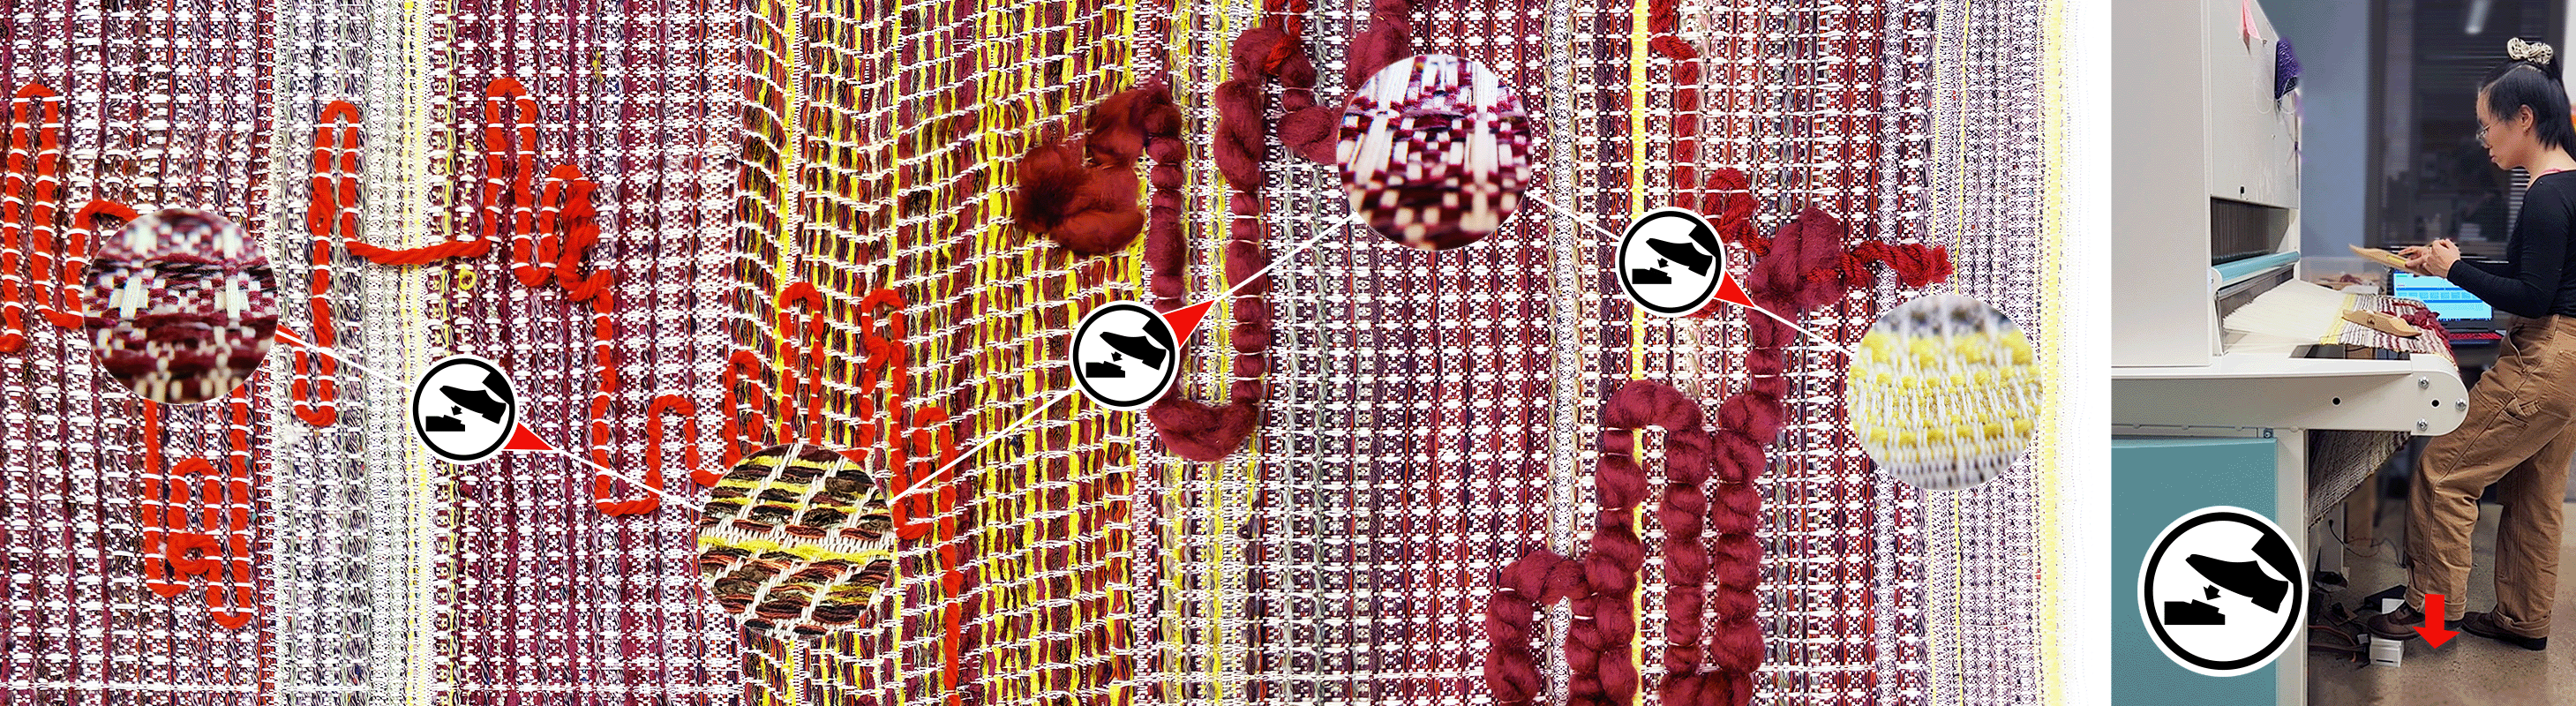
\includegraphics[width=\textwidth]{figs/LP_teaser-v2_SMALL.png}
%     \caption{A large project woven by one of the authors using the Loom Pedals prototype interface for Jacquard weaving. The system of modular, reconfigurable foot pedals allows the weaver to improvise a design without a pre-prepared file. In the sample shown, the weaving began on the leftmost edge and progressed from left to right. By assigning functions which generate and transform woven designs to each pedal, the user can playfully design the fabric at the loom by choosing a sequence of pedals to step on. Foot pedal icon by Daniel McDonald from the Noun Project.}
%     \label{fig:teaser}
% \end{figure}

% \section{Introduction}
\label{ch_lp_intro}

A growing body of research in emerging technologies is recognizing the value handcraft and textile technologies can bring to the world of computing; for example, the creation of "the first computer" traces back to weaving, in the form of the Jacquard loom. \cite{harlizius-kluck_weaving_2017} Further technological inspiration can be found scouring textile histories. From sustainable fabrication, where an array of compostable materials like grass, reeds, or animal hair can be woven into garments, to wearable technologies that regulate body temperature or augment our range of communication, we find there is a wealth of wisdom stored in crafts. Yet, historical exclusion of textiles from what is considered high tech, and marginalization of those who preserve handcraft traditions, especially Indigenous communities and women \cite{flores_weaving_2021, muskrat_magazine_indigenous_2013, rosner_making_2018}, demands that we attend to these troubled power dynamics when working at the intersection of computing and textile technologies.

In this work, we challenge one notion of high tech weaving and examine value that has been overlooked in older, more traditional textile technologies. Specifically, we compare Jacquard weaving with weaving on a traditional wooden floor loom. Weaving can be accomplished on many kinds of looms. But most often, the complex weaving required by HCI uses a particular model: the TC2 Digital Jacquard loom, one of the only prototype-scale Jacquard looms on the market. TC2 looms allow a designer to upload a set of machine instructions for making cloth in the form of a bitmap image. After sending this image to the loom, it is interpreted by raising the warps indicated by the location of black pixels on the bitmap. A weaver inserts the yarn then steps on a foot pedal to advance to the next row in the predetermined file. Revisions to this process are costly: the weaver must leave the loom, return to the design file, reformat the bitmap, and send the file back to the machine before starting again. 

Not only can this workflow slow iterations and prevent rapid prototyping, it disrupts the creative process traditionally present when weaving; weavers cannot respond to their materials or explore alternate possibilities. In other looms, patterns are algebraically encoded into frames, playfully combined, and manipulated to give rise to emergent outcomes. In these models, the weaver has multiple choices they can make at each row while weaving. Harlizius-Kl\"{u}ck states in her deconstruction of the Jacquard-as-computation narrative: “Jacquard’s cards are the end of this story [of weaving evolving algebra and computation], rather than its beginning, reducing the weaving from a coder of weaves, to an operator who had to step on a single [foot pedal] repeatedly." \cite{harlizius-kluck_weaving_2017} This playfulness is a key part of the creative process characterizing the ingenuity of weavers. 

These observations inspired us to confront the frustrations we had personally encountered when attempting to weave playfully with a Jacquard loom. Drawing from our own weaving practices to situate our inquiry, we sought to design an interface for a TC2 Digital Jacquard loom to enable creative improvisation. We found ourselves taking inspiration from pedals and levers used in other kinds of centuries-old looms, as well as technologies from other domains, namely musical foot pedals and related hardware. In the following paper, we present the Loom Pedals system that emerged from our prototyping process as a case study about augmenting an existing computer-controlled loom to invite improvisational and open-ended play. 

Because the history of loom design informed our novel interface, we contextualize the work by reviewing different types of looms and how traditional looms influenced our design for modern Jacquard weaving. Next, we detail our design process, and the metaphors that helped guide it, before delving into the experience of using the Loom Pedals prototype. We then reflect on what those experiences taught us about play, as it relates to weaving, and report on possible future directions and explorations for the Loom Pedals system.

Our contribution consists of: the Loom Pedals prototype, source code, and bill of materials as an open-source project, the findings from our design inquiry, and the review of various loom mechanics, as a source of inspiration for researchers interested in weaving and craft. Specifically, we present our inquiry as a novel case study of augmenting existing equipment through peripherals informed by historical technologies. 
% By enabling playful interactive fabrication, we found that this human-machine collaboration enlivened the . 
We hope that our experiences will inspire readers to also investigate weaving as both craft and technology – joining us in a web of warp and weft, humans and machines, digital and analog, histories and futures.

\section{Related Work}
\label{sect_related-work}

Here, we review other works from HCI and digital fabrication that explore weaving, situating our research amongst the creative and technological interests of our community. 

\subsection{Weaving in Digital Fabrication}

Textiles have been a rich domain for digital fabrication to explore, offering techniques, besides weaving, such as: knitting \cite{mccann_compiler_2016}, crochet \cite{okazaki_metamocrochet_2014}, spinning yarn \cite{rivera_desktop_2019, studio_hilo_open_nodate}, and embroidery \cite{jo_skinlace_2021}. Technologists have used these techniques to create novel artifacts like soft robotics \cite{luo_knitui_2021} and e-textile circuitry \cite{posch_crafting_2017}. Using weaving, researchers have leveraged its complex, grid-based structures to create sensors \cite{pouta_woven_2022, devendorf_introduction_2022} and wearable devices \cite{huang_wovenprobe_2021, sun_style-woven_2022}. Its diversity of methodologies can even generate 3D objects, such as garments \cite{mcquillan_hybrid_2019} and multi-layered folding shapes \cite{richards_weaving_2012, mayer_clothing_1984}.

From an HCI perspective, these works have renewed interest in textile crafts, by introducing traditional practices into the realm of computing research. Besides crafted items, researchers have also investigated craft processes themselves. Works like EscapeLoom \cite{deshpande_escapeloom_2021}, personal Jacquard weaving \cite{albaugh_enabling_2021}, and open-source DIY looms \cite{noauthor_frame_2017} consider the potential benefits of digital fabrication for making novel, accessible weaving tools. Furthermore, a growing domain of interactive fabrication and flexible fabrication leverages both the complex machinery of weaving, 3D printing, and other techniques, while recognizing the value of a human designer’s participation in making \cite{albaugh_investigating_2020, gifford_systems_2015, kim_compositional_2018, sun_flextruss_2021}.

\subsection{Textile Crafts, Technology, and Design}

Weaving – as an embodied process, cultural practice, even political statement – has been a provocative action for many designers. In HCI, Fernaeus et al. investigated a mill with original, wooden Jacquard looms, dating back to the Industrial Revolution, and found design lessons for modern computers in the looms’ longevity and historical uses \cite{fernaeus_revisiting_2012}. A collaborative study conducted by Zhang et al. with communities of Malaysian Songket weavers offered insight into the innovation embedded in grassroots infrastructures and highlighted the value of tradition in this sociotechnical context \cite{zhang_designing_2019}. Finally, Oogjes et al. reflected on the bodily experience of weaving as part of a human-machine-material ecological network \cite{oogjes_weaving_2022}, providing language for our own practices of noticing, thinking, and making. 

We characterize these aforementioned works, or specific artifacts, as case studies that explore themes shared in this research. More broadly, we look to methodologies such as autobiographical design \cite{neustaedter_autobiographical_2012, desjardins_revealing_2018}, embodied interaction and somaesthetics \cite{hook_unpacking_2021, baurley_modalities_2020, vaughan_embodying_2006}, as well as embodied knowledge and craft-based inquiry \cite{flanagan_tracing_2019, frankjaer_understanding_2018, schoemann_needle_2017} to immerse ourselves in our subjective experiences and to understand the role of weaving in generating our design. While our work does not directly engage with the sociopolitical dimensions of weaving, we strove to honor how crafts and textiles have been historically devalued as low tech knowledge, and how textile traditions are vehicles of resilience and political resistance for Indigenous communities \cite{flores_weaving_2021, montero_spinning_2021}

\subsection{Improvisation and Playfulness in Fabrication}

As interest in digital fabrication has grown over the last several years, so too have discussions that explore how to integrate chance, playfulness, and otherwise improvisational experiences into the making process. Early projects in interactive fabrication, such as Constructable \cite{mueller_constructable_2013} and Protopiper \cite{agrawal_protopiper_2015}, sought to enable improvisation by offering direct manipulation to the design in-progress, like using a laser pointer to modify a laser-cut design on-the-fly. Others frame improvisation as inviting various forces to participate in the design and creation process, augmenting the voices of the machine and/or materials. Threadsteading \cite{albaugh_threadsteading_2016} and Exquisite Fabrication \cite{goveia_da_rocha_exquisite_2021} show how playfulness can be applied literally as well, by integrating games into the making process. 

Playfulness can also be subversive, because these projects prioritize unexpected outcomes, rather than conventional fabrication metrics like precision and throughput. For instance, Dew \& Rosner's work in timber construction focused on living materialities as part of making, which meant the post-making process of the materials' decay became a factor as well \cite{dew_lessons_2018}. Similarly, recent fabrication research has examined unmaking as a valuable kind of interaction \cite{song_unmaking_2021}, creating a dialogue between fabrication and sustainable design and materials. Overall, these projects frame improvisation as an interaction between humans and technology that can foster deep material engagement. 

Our study participates in this larger conversation regarding play as it applies to looms, of many origins and uses, as a kind of human-machine cooperative interface of interest. It does so by augmenting these systems with hardware peripherals that are aimed at inviting playfulness and embracing improvisation within the traditionally rigid process of Jacquard weaving.

\section{Loom Hardware and the Weaver's Design Process}
\label{sect_bg-looms}

\begin{figure}[h]
  \centering
  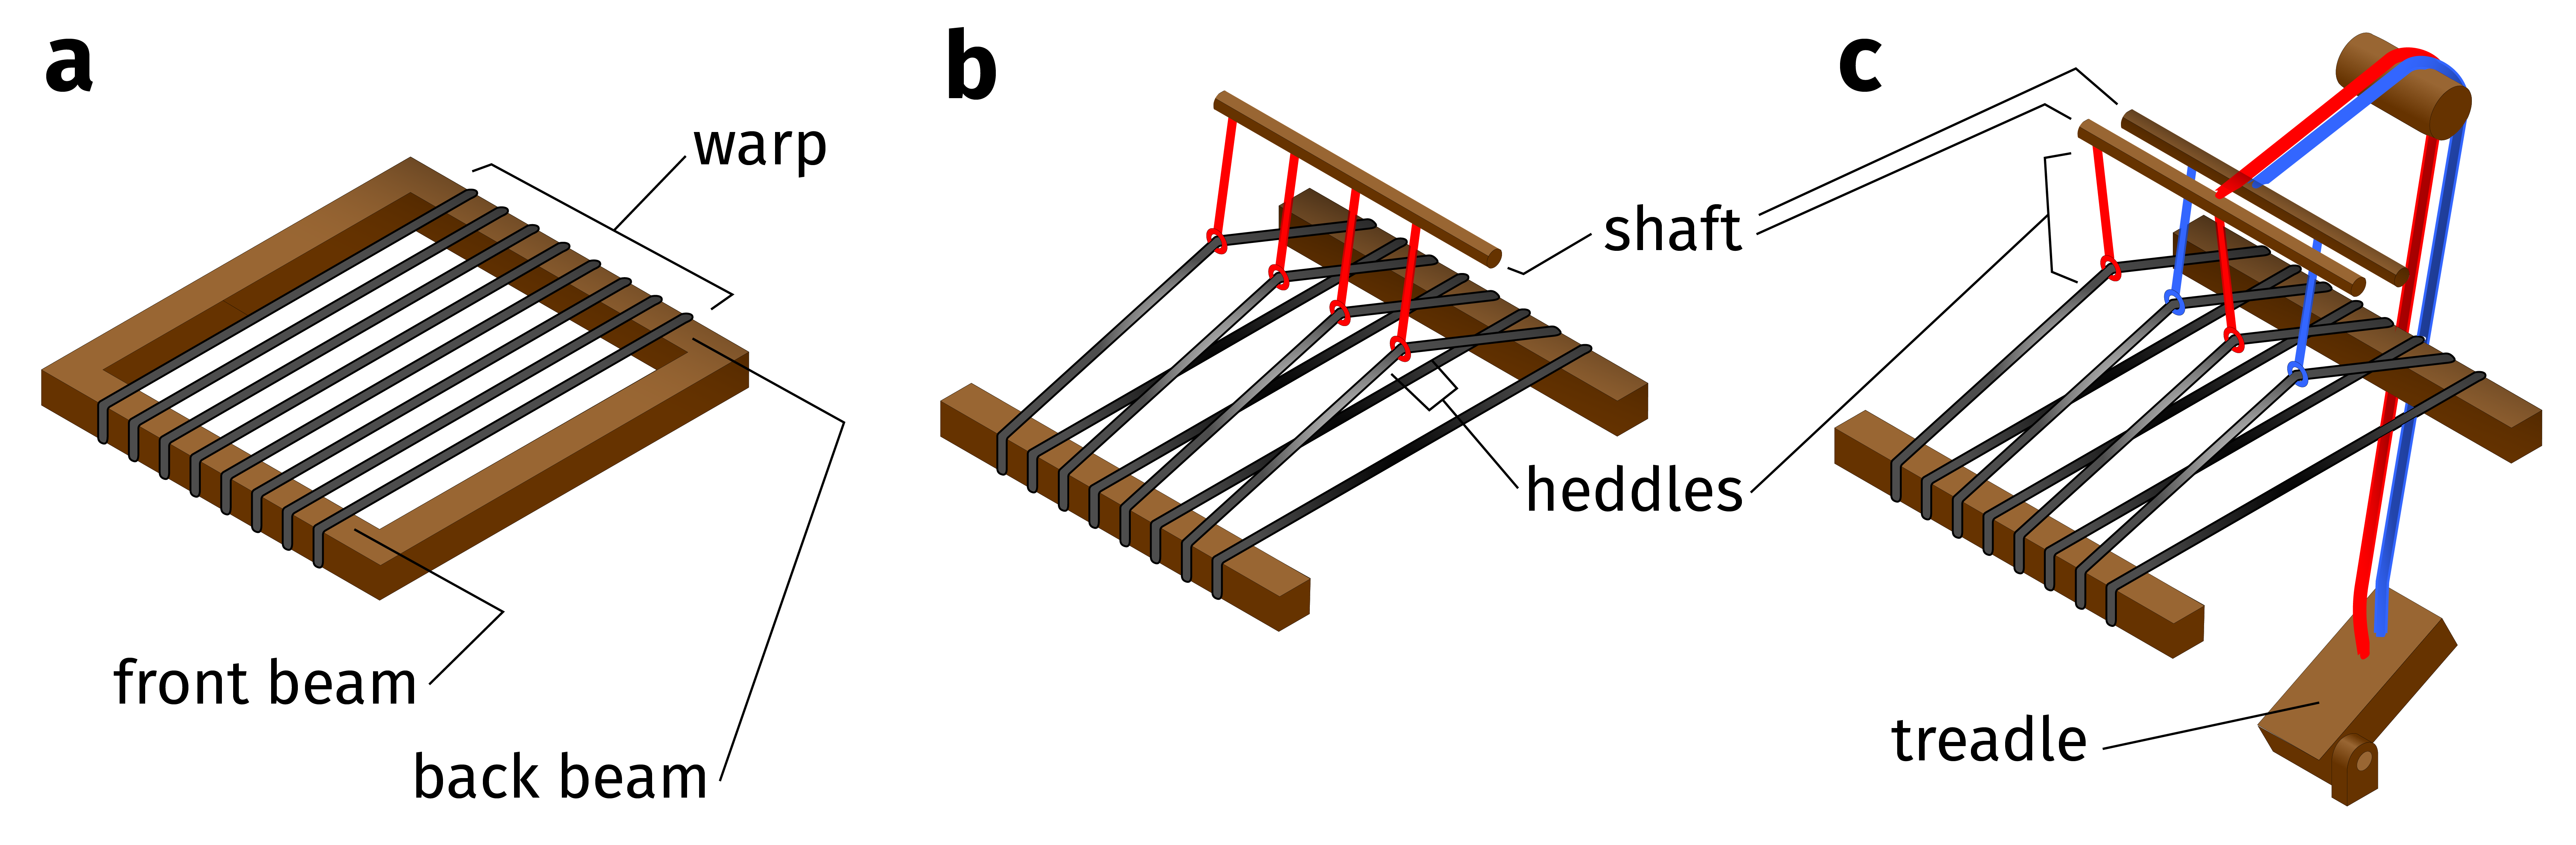
\includegraphics[width=\linewidth]{figs/LP_2_loom-parts.png}
  \caption[Illustrations of different hardware components of weaving looms.]{Simplified cartoons that illustrate each of the weaving hardware components discussed. (a) A loom that consists of a frame with two beams holding the back and front of the warp, equivalent to a tapestry loom. (b) A loom with one shaft that lifts half of the warps with one motion, using heddles around the selected warps, equivalent to rigid heddle looms and many backstrap looms. (c) A loom with two shafts, both tied to one treadle, which will lift the same shed as in (b). However, now it is possible to select which shafts are associated with the treadle, equivalent to shaft or frame looms.}
  \label{fig:loom-parts}
\end{figure}

Our experiences weaving on other types of looms, primarily multi-shaft floor looms (henceforth referred to as shaft looms), motivated us to modify the physical interface of a Jacquard loom. Because our arguments hinge upon how weaving on these looms physically compares to weaving on the TC2 digital Jacquard loom, we will first review the core mechanics of weaving looms and compare possibilities for design and play across different types of looms. We will focus on three in particular: tapestry, shaft, and Jacquard looms.

\subsection{Tapestry Looms}

In general, looms are machines for weaving: interlacing sets of yarns to create fabric. The oldest and most fundamental loom mechanism is a frame that holds one set of yarns, the warp, in place, so that the weaver can interlace a perpendicular set of yarns, the weft, into the desired structure. Tapestry looms only require this basic frame (Fig. \ref{fig:loom-parts}a), and thus, are sometimes called ``frame looms". A tapestry weaver creates fabric by manually manipulating the weft and warp, often with their fingers and a large needle \cite{mezoff_art_2020, moodie_loom_2016}. In essence, a tapestry loom allows one to draw free-hand with yarn, creating different imagery and textures. Consequently, tapestry weaving tends to incorporate long loops, knotted fringe, twists, and other textured structures beyond strict over-and-under weaving \cite{rousseau_contemporary_2023}. The loom's simplicity imposes very few constraints on how the weaver's hands can move in and out to manipulate the yarns, encouraging these unusual techniques.

\begin{figure}
    \centering
    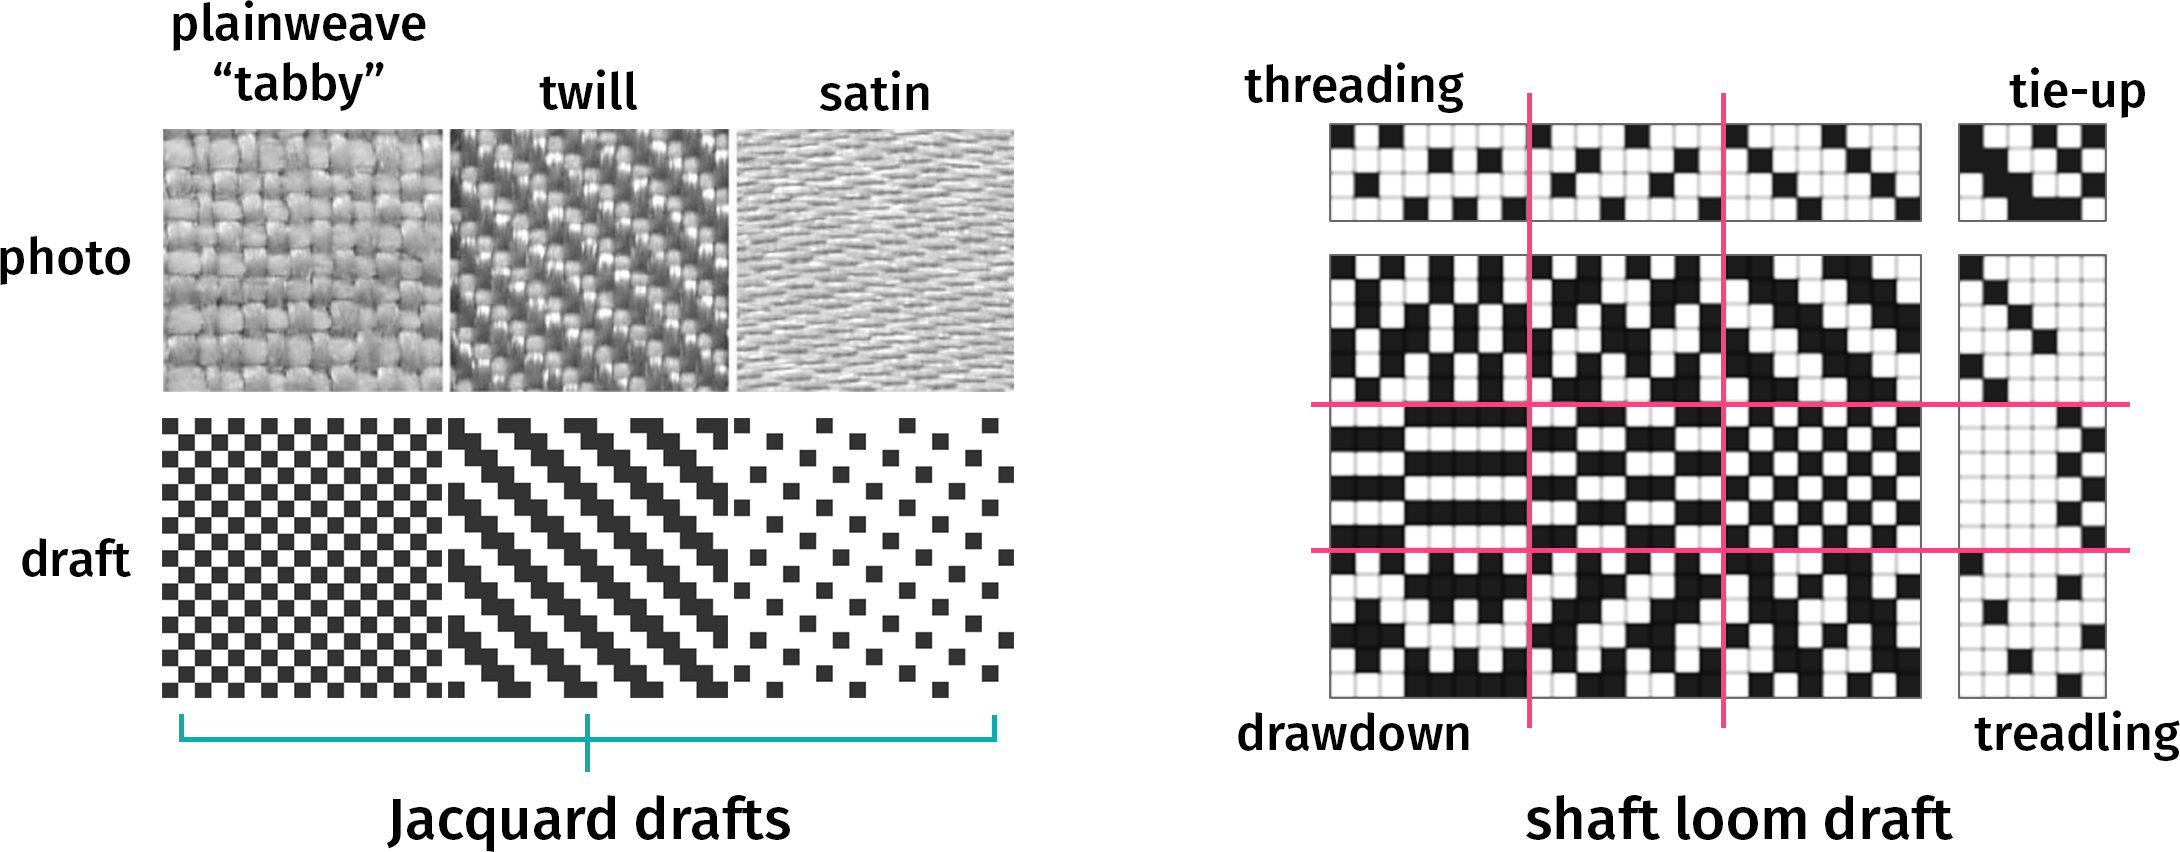
\includegraphics[width=0.7\linewidth]{figs/LP_3_drafts.png}
    \caption[Overview of weaving drafts and how they differ across looms.]{Overview of drafts in weaving and how they represent the cloth’s structure as well as the fabrication method. (left) Comparisons of three common weave structures (plain weave, twill, and satin) in photos of the cloth, as well as their drafts. The drafts are formatted for Jacquard looms. (right) A draft for shaft looms that shows the additional sections required: threading, tie-up, and treadling. The upper-right section is a draft for the same twill structure in the Jacquard draft. The other sections demonstrate how changing the threading or treadling can dramatically alter the woven structure.}
    \label{fig:drafts}
\end{figure}

\subsection{Shaft Looms}

Shaft looms introduce two mechanisms to the basic frame. The first are heddles, grouped into sets, which share common shafts \cite{broudy_book_1993}, allowing the weaver to simultaneously lift a set of warps and quickly pass the weft through (Fig. \ref{fig:loom-parts}b). The second are treadles, foot pedals which can lift multiple shafts (Fig. \ref{fig:loom-parts}c). When setting up their loom, shaft loom weavers first choose a threading by assigning each warp to one of the shafts \cite{chandler_learning_2009, osterkamp_weaving_2005}. Both shaft loom and Jacquard weaving designs rely on interlacing wefts over and under the warps in specific patterns. These patterns, represented by drafts, also denote different woven structures and fabric properties, as seen in Fig. \ref{fig:drafts}. 

\begin{figure}
    \centering
    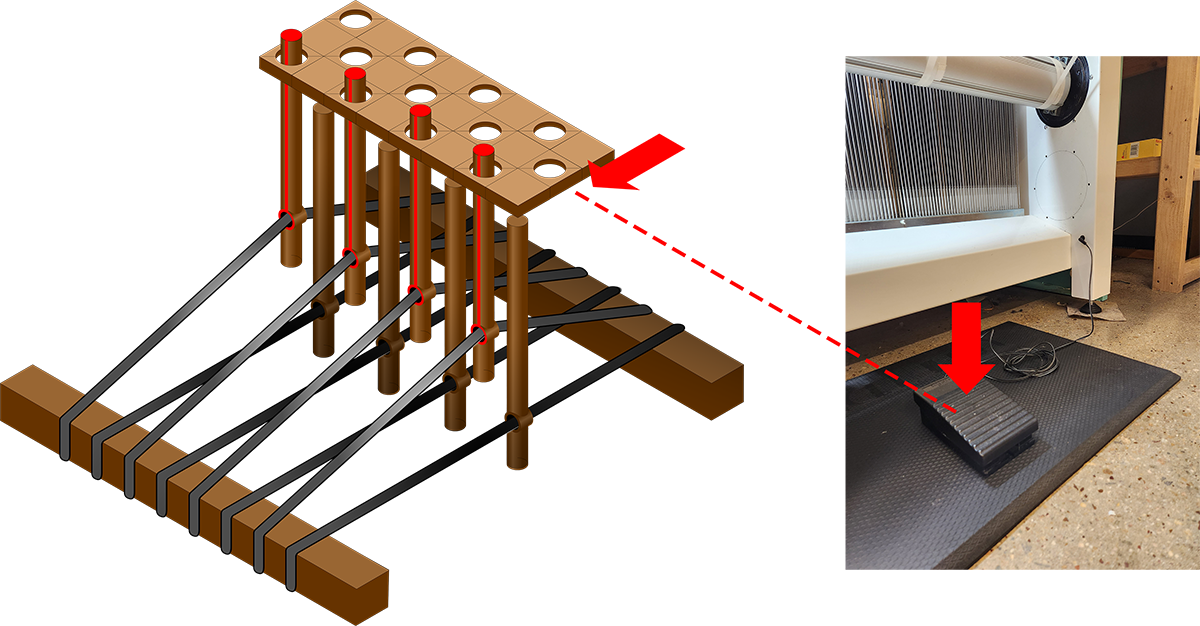
\includegraphics[width=0.6\linewidth]{figs/LP_4_jacquard-loom.png}
    \caption[Visualization of a simplified Jacquard loom.]{Visualization of a simplified Jacquard loom. The Jacquard mechanism is abstracted away as an invisible component that can control each heddle individually. The arrow indicates the direction that the punch card progresses to the next row of the draft. In the existing TC2 interface, a foot pedal (right) advances the draft with each step.}
    \label{fig:jacquard-mech}
\end{figure}

Shaft loom drafts are divided into four sections (Fig. \ref{fig:drafts}b) to convey specific combinations of the treadling, tie-up, and threading, indicating the shafts each warp lifts. Weavers can change their treadling, meaning the sequence of treadles they step on, to achieve a completely different woven structure \cite{kesler-simpson_creative_2021}. Furthermore, weavers can quickly alter their loom’s tie-up by unhooking or untying the cords for each shaft, and selecting a new combination of shafts for each treadle by reattaching these cords. The integration of heddles, shafts, and treadles allows weavers to experiment with different structures and flexibly iterate upon their designs, giving rise to complex woven patterns with fairly simple hardware. 

Because of the somewhat magical interplay of materials, threadings, and different treadling options, the constrained pattern space of shaft looms creates room for exploration and experimentation. For some weavers, this ability to play with different derivations between a single structure can inspire lifelong careers and explorations \cite{kesler-simpson_crackle_2022, franklin_weaving_2018}. It should also be noted that tapestry and hand techniques have been integrated into shaft loom weaving; however, these techniques are less prevalent due to the assumptions built into the machine for weaving linear and repeating patterns. 

\subsection{Jacquard Looms}

Jacquard looms enable even greater complexity in woven fabrics by exchanging shafts and treadles for the Jacquard mechanism, which lowers and raises each yarn independently, rather than in fixed sets (illustrated in Fig. \ref{fig:jacquard-mech}). A weaver executes a design on a Jacquard loom by loading the draft into a punch card, or a digital bitmap equivalent, then inserting the card into the machine to be read row-by-row \cite{fernaeus_revisiting_2012}. (Fig. \ref{fig:drafts}) This system opens up a much larger possibility space for woven design, as the Jacquard loom can lift warps in any arbitrary pattern \cite{holyoke_digital_2013, ng_innovative_2013}. Where some Jacquard looms are entirely automated, others, like the TC2, use the Jacquard mechanism to control the warp pattern, while relying on the weaver to physically insert the weft yarns. 

The current workflow of the TC2 digital Jacquard loom asks the weaver to act as the print head on a predetermined file. This leaves room for the weaver to apply hand/tapestry techniques within the emerging cloth or play with inserting different materials and observing their behaviors. Manual involvement in this process offers design possibilities and textures that are unobtainable in fully-automated weaving. That said, Jacquard weaving, compared to shaft looms, requires much more time to plan the draft. Designing a Jacquard draft often asks the weaver to assemble their pattern without knowledge of how their materials will behave \cite{schlein_woven_2007, ng_innovative_2013}. Should one want to change their pattern, they must enter a laborious cycle of redesigning and reuploading their file before restarting the weaving process. This does not make improvisation impossible; but it does impose a significant time cost. 

\subsection{The Broader Space of Looms}

While our design was most heavily inspired by the looms described above, it is worth noting that this history of loom design presents only a small subset of the mechanisms and equipment used for weaving. Looms such as warp-weighted looms and backstrap looms have been used longer than there is written history \cite{pritchard_crafting_2022, postrel_fabric_2020}. They have encoded patterns in the body, song, and environment, and require collaboration amongst multiple parties \cite{tuck_singing_2006, rebay-salisbury_knowledge_2014}. Some of these looms are portable, some are made with found materials; each brings its own unique approach to encoding and reproducing patterns. We believe this history can be of interest to the HCI community as it shows multiple different methods for making cloth, each uniquely configuring humans, machines, and materials in the computational process of weaving. 

\section{Design Process}

In this section, we provide the conceptual framing of our prototype system, informed by the mechanisms discussed above. We elaborate on the current workflow for Jacquard weaving design, the existing TC2 interface, and the main frustration points in the design process. We then describe the design methods and metaphors which informed our work and subsequent reflections.

\subsection{Design Goal: Improvisation and Play in Weaving}

In the context of weaving, we define improvisation as the ability to begin weaving immediately, no planning or draft required, so the weaver is free to alter the design while using the loom. Thus far, we have discussed how looms differ in mechanical complexity, which influences how weavers design for each type of loom. In general, more complex looms are less conducive to improvisation. Current Jacquard workflows emphasize a large possibility space, while sacrificing ease of alteration, as adjusting or manipulating the design requires the weaver to prepare a new punch card or image file. 

On the other extreme, a tapestry weaver has complete freedom to weave any structure at any point in their design process. Shaft looms fall in the middle of this spectrum, offering several options for altering a design on-the-fly. Without reconfiguring any part of the loom, the weaver can change designs by changing their foot movements. For an even greater shift, the weaver can rearrange their tie-up. The only fixed mechanical configuration on a shaft loom is the threading, not the entire draft. Yet even the threading process presents opportunities for improvisational play, as weavers can experiment with different colors and textures in the warp \cite{essen_easy_2016}.

When on the loom, weaving a sample cloth, known as sampling, is not only crucial for testing and refining a design, but is also one of the main sites for play during weaving. In the words of Amanda Rataj, a contemporary weaving instructor, ``sampling is like making a sketch---you learn more about your materials\ldots{}and how the finished textile behave\ldots{}[But it] isn’t all just about practical weaving knowledge---[it’s] also about having fun and trying something I wouldn’t typically make." \cite{rataj_tips_2020}

With these facets of playful weaving in mind, our design prioritizes: \textit{reconfigurability}, lowering the cost of making changes, and \textit{modularity}, in the form of sampling functions that can quickly generate ideas.

\subsection{Existing TC2 Interface, Sampling Workflow, Frustration Points}

In the decade since its release, the TC2 loom has accumulated a worldwide community of users, ranging from independent artists, to industry researchers, and academic institutions. The TC2's design process is typical for a Jacquard loom; designers use computer-aided design (CAD) software, e.g. Arahweave \cite{arahweave_2023} or JacqCAD \cite{jacqcad_2019} to prepare their Jacquard draft. First, the designer creates a digital image file, then defines regions in the fabric corresponding to different features, and finally fills the regions with the desired weave structure \cite{holyoke_digital_2013}. Afterwards, the designer takes their file to the loom. TC2 users most commonly use Adobe Photoshop for their drafts, loading their weave structures as Photoshop Patterns \cite{schlein_woven_2007}.

To sample a project on the TC2, a user weaves a representative slice of their larger draft, in order to test the chosen structures, materials, and resulting cloth. If the weaver wants to adjust their design after sampling, they must leave the TC2, return to the design software to remake their draft file, which may take hours, then re-sample the revised draft. Beyond that, this workflow assumes that the weaver has already developed an idea enough to create the initial draft. In both our own experiences, and those of other TC2 weavers we have spoken with, this iterative sampling process is generally tedious and frustrating. Often, more time was spent working in editing software than at the loom. By separating the file design and fabrication phases, this workflow was also severing the generative relationship between designing and making in handloom weaving.

\subsection{Conceptualizing the Loom Pedals}

\textbf{How can we bring improvisation into Jacquard weaving through the loom’s user interface, and what experiences or possibilities emerge in designing such a system?} We implemented the Loom Pedals as one possible answer to this question, allowing us to develop and study the emergent practices with such a tool. Here, we give an overview of the overarching methods and conceptual metaphors that informed our design research. 

\subsubsection{Methods}

We looked to craft-based design inquiries in HCI to guide our research, with a particular emphasis on “creating knowledge through deep, embodied engagement" \cite{frankjaer_understanding_2018}. Working with these principles directed us at first towards autobiographical design \cite{neustaedter_autobiographical_2012, desjardins_revealing_2018}, where our own embodied weaving experiences would shape the design of the Loom Pedals. However, we never envisioned this research happening in isolation. We sourced ideas from crafters and artists who spoke of their own embodied experiences with weaving and textile design: such as Harlizius-Kl\"{u}ck’s writing on the algebraic complexity of shaft looms. We also valued input from our own community of practitioners, which led us to seek their ideas through collaborative design \cite{devendorf_craftspeople_2020, mironcika_snap-snap_2020, recupero_balancing_2021}.

\subsubsection{Design Metaphors}

Two metaphors emerged during the Loom Pedals' design process which helped clarify both improvisation and play as they relate to weaving, namely: \textit{weaving as music} and \textit{weaving as conversation}.

Throughout this paper, we reference musical concepts and practices, to reflect how several design choices were directly informed by drawing such comparisons between weaving and music. For example, we considered why improvisation felt easier when weaving on a shaft loom, and in doing so, developed a conceptual model of improvisational weaving. Treadles were key, as they provided a well-defined set of choices for the weaver. In the same way musical notes within a given key form chords, treadles enable a woven pattern to emerge from sequences of treadling steps. 

The second metaphor of \textit{weaving as conversation} considers how several facets of our research were fluid processes, in which multiple agents responded to one another. We are not the first to investigate fabrication as a conversation between humans and the more-than-human \cite{kim_shall_2017, kim_machines_2017}, such as the rhythmic movements of a weaver's body interacting with the loom's mechanisms while weaving. At the same time, we utilized direct communication between weavers, like altering a design tool's interface in response to user testing. Both play a role in the complex dialogue weaving engages us with. 

\section{Loom Pedals System}

In this section, we describe the basic functionality of the Loom Pedals interface that blends the design and fabrication phases of Jacquard weaving. Inspired by musical effects pedals, where several types might be used during a performance to achieve different effects, we sought to explore the concept of multiple hardware inputs in the context of weaving. Therefore, we designed the Loom Pedals system to handle any number of connections, each configured to a unique function to be applied when weaving. Similarly, we chose pedals as the form factor due to this comparison, as well as the pre-established singular foot pedal in Jacquard weaving. Figure \ref{fig:sys-connections} gives an overview of the architecture of hardware, communication protocols, and software user interface that resulted.

\subsection{Weaving with the Loom Pedals}

\begin{figure}
    \centering
    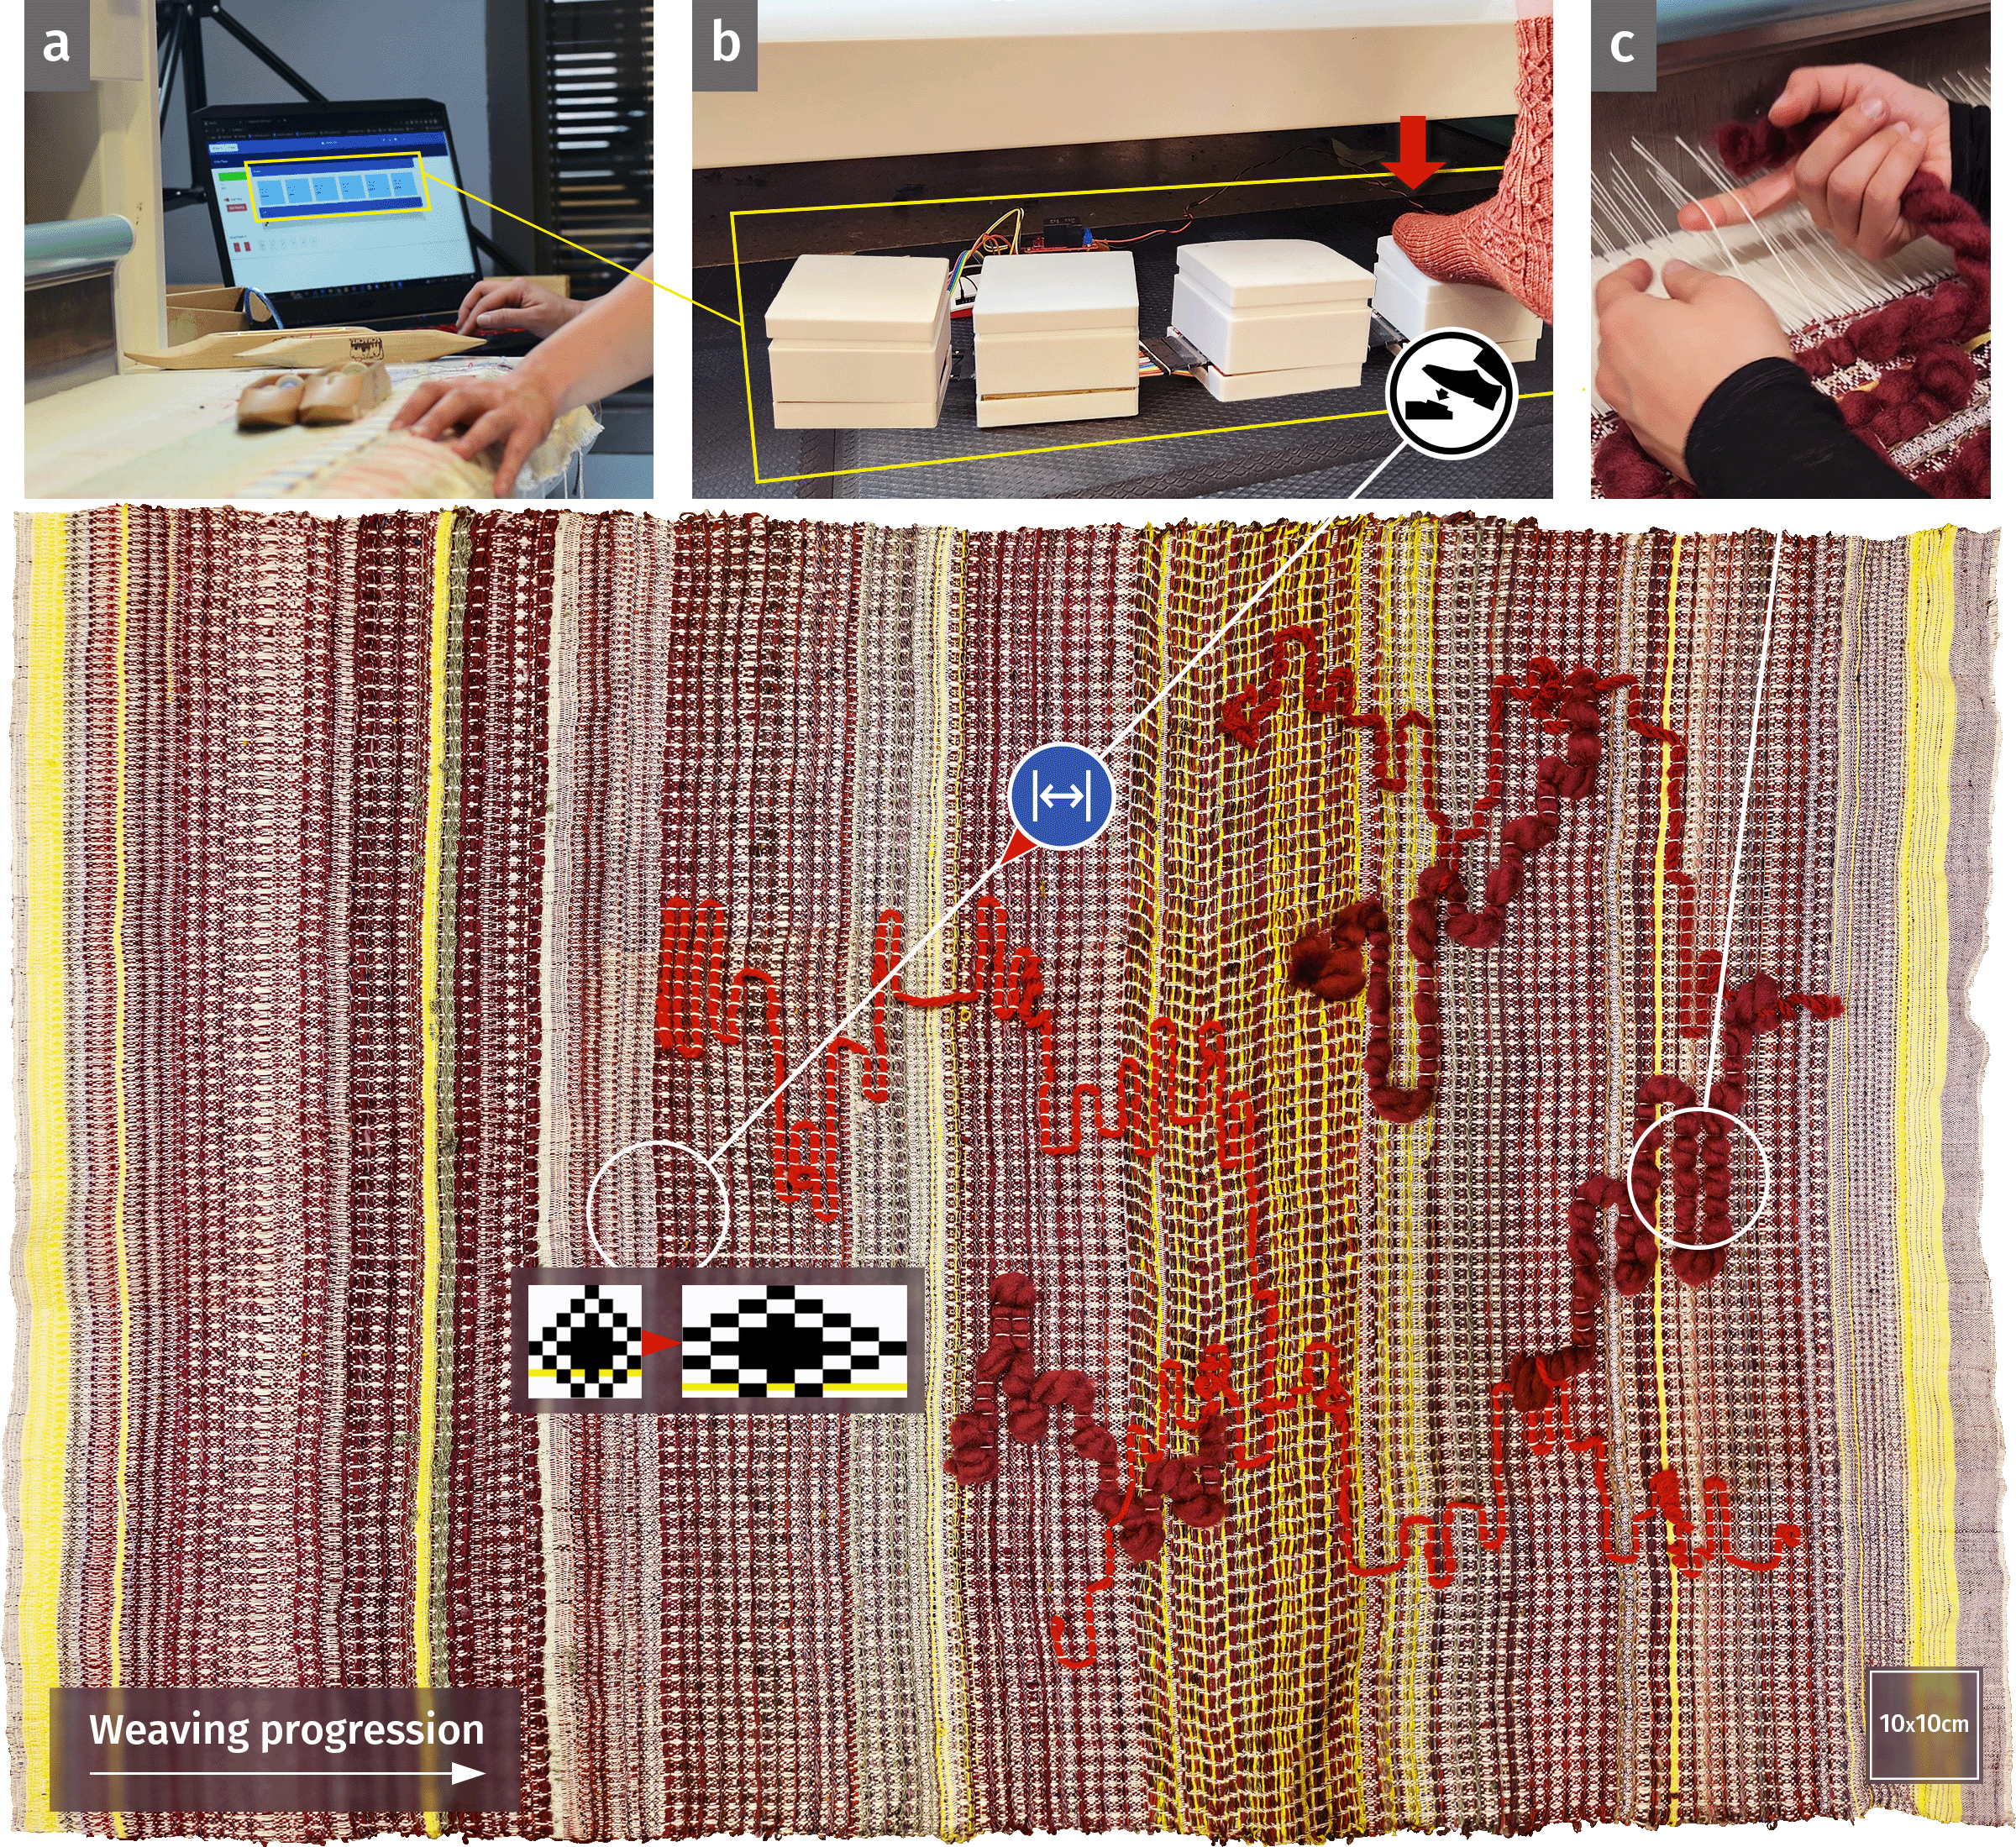
\includegraphics[width=\linewidth]{figs/LP_fig_workflow_SMALL.png}
    \caption[Key user interactions for the Loom Pedals weaving workflow.]{Key user interactions for the Loom Pedals weaving workflow. a) Before starting a weaving session, the user configures the number of Pedals connected to the system and assigns functions to each Pedal to control design edits and weaving progression. b) While the user is weaving, they can step on a Pedal at any point to execute the assigned editing function. In this example, the user stepped on a Pedal that will horizontally stretch the draft, and the point in the fabric reflecting this change is indicated. c) With these interactions delegated to their feet, the user is free to use their hands to enact even further improvisational experiments while weaving, such as manually inserting a freeform yarn accent, like a tapestry weaver.}
    \label{fig:example-workflow}
\end{figure}

Broadly, the Loom Pedals system consists of three components: the Pedals, the TC2 digital Jacquard loom, and the design interface software used to communicate between the two. To accompany the following walkthrough, we also present an example workflow using the Loom Pedals in Fig. \ref{fig:example-workflow}, documented while evaluating the system by weaving a large project.

To begin weaving with the Loom Pedals, the weaver first powers on the TC2 and connects it to the Draft Player design interface. Additionally, they must physically connect the Loom Pedals to the TC2 and prepare their desired yarns. If they have a pre-made design file, they can load the file directly into the Draft Player; otherwise, they can select from a list of draft presets. While in the Draft Player window, users can map an Operation to each Loom Pedal currently connected. These Operations execute when the weaver steps on a given Pedal and alter the draft in some way. For instance, using the Loom Pedals, a weaver can: flip their draft, increment its scale, activate or deactivate certain yarns in the design, etc. 

Once each Pedal is configured, weaving can commence, either by pressing the start weaving button in the Draft player or stepping on a Pedal mapped to the start/stop function. This signals the TC2 to lift the first row of the draft and the weaver can now pass the shuttle through to weave that row. From here, the weaver can choose to progress through the draft as normal, sending each row to the TC2 and weaving it, or they can start reshaping the draft using the Loom Pedals. Before sending a row to the loom, the weaver is now presented with a number of choices regarding which transformations they wish to apply. Navigating these options and making spontaneous decisions, while in the process of weaving, is the primary interaction loop of the Loom Pedals. The result is a more improvisational and playful kind of weaving, one which engages the weaver in a dialogue between themselves, the loom, and their own imagination.

\begin{figure}
    \centering
    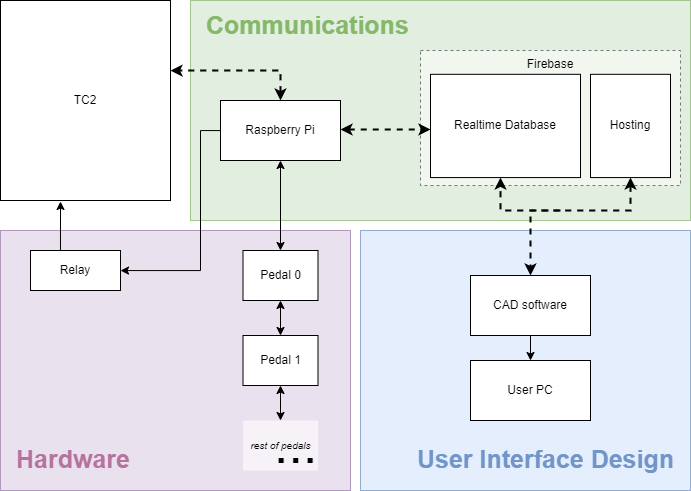
\includegraphics[width=0.8\linewidth]{figs/LP_5_sysConnections.png}
    \caption[Overview of Loom Pedals system components.]{Overview of how the system components connect to the TC2 and with each other. Lines with only one arrowhead indicate one-way communication between components (output to input). Dashed lines represent wired communications (via TCP/IP or other networking protocols). While solid lines represent wired connections between components.}
    \label{fig:sys-connections}
\end{figure}

\subsection{Hardware: Circuit and Physical Design}

The following sections of technical description will be brief. More detailed documentation, as well as our source code, circuit schematics, CAD files, Jacquard drafts, and other assets can be found on Github \footnote{See Appendix \ref{apx_git}.} and will be updated as development on the Loom Pedals continues.

To ensure flexibility in our modified TC2 workflow, weavers are able to add or remove Pedals and customize the functions according to their preferences. The Loom Pedals are reconfigurable and interchangeable due to the digital logic circuit built around each Pedal module's physical switch. Each module can be connected in a chain, with only the first Pedal directly connected to the controller: a Raspberry Pi. Additionally, the controller receives a count of how many Pedals are in the chain, as well as the input state of each one. This design minimizes the effort required by the user to add or remove pedals, as they only need to (un)plug one end.

\begin{figure}
    \centering
    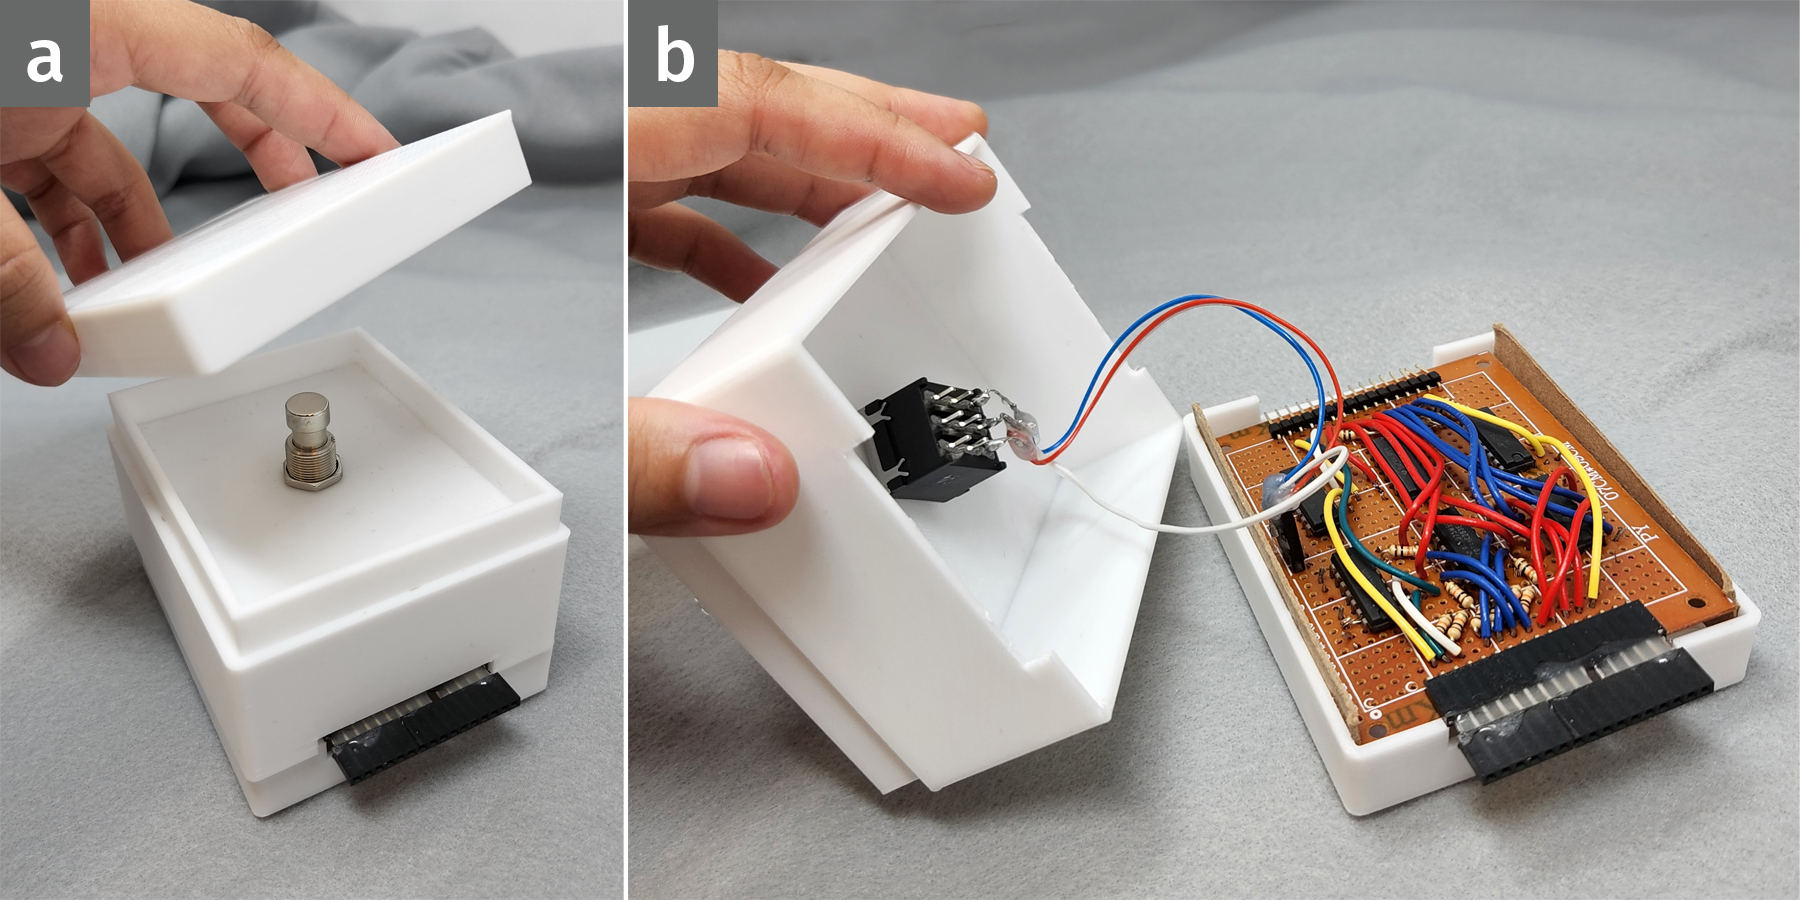
\includegraphics[width=\linewidth]{figs/LP_6_pedal-enclosure.jpg}
    \caption[Photographs of a single Pedal module.]{A single Pedal module and its physical enclosure, consisting of (a) a top plate that covers the foot switch and (b) a lower box which both secures the switch and houses the circuit board. The enclosure includes slots on two of the sides to connect Pedals to each other interchangeably.}
    \label{fig:pedal-module}
\end{figure}

Our prototype shown in Figs. \ref{fig:pedal-module} \& \ref{fig:connecting-pedals} implements the circuitry using discrete IC’s, that were manually soldered to a perfboard. While we have since designed and printed custom PCB's for later iterations, we present this early version without custom electronic components to pay homage to musicians who similarly build their own pedals ``from scratch" \cite{collins_handmade_2020}. The Pedals use 3PDT stomp switches, the same hardware that is commonly used in these musicians' DIY pedals. In addition to the Pedal modules, the hardware includes a power relay, also controlled by the Raspberry Pi, which connects to the TC2 in place of the existing foot pedal. This relay ensures that user inputs are correctly sent between the TC2 and the Pi.

Our preliminary design for the Pedal enclosures consists of: a top panel for ease of stepping and a case to mount the switch, with the circuit board underneath (Fig. \ref{fig:pedal-module}). We categorize portions of the circuit assembly as part of the physical design because the circuit boards include header connections on either side, so that the user can add/remove Pedals by physically attaching modules. 
% Accordingly, the case has openings on each side to enable these connections.

\begin{figure}
    \centering
    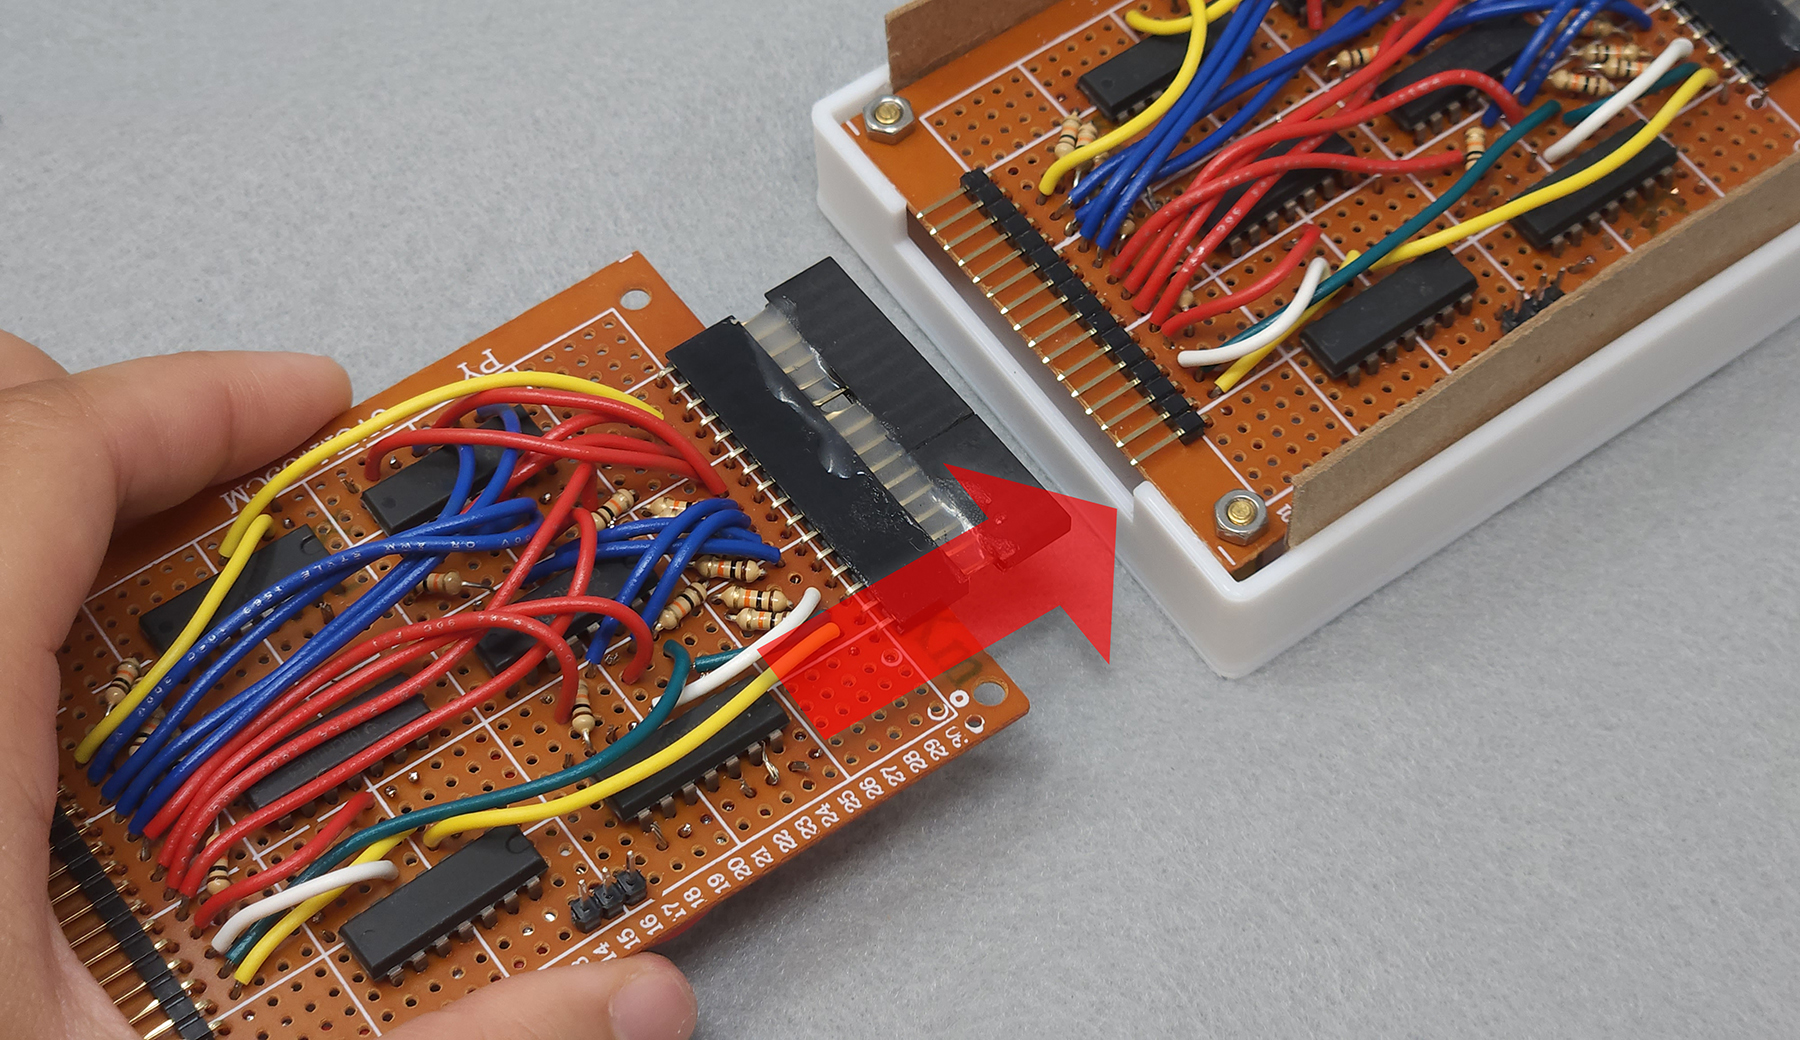
\includegraphics[width=0.6\linewidth]{figs/LP_8_connecting.jpg}
    \caption{Two Pedal circuit boards connecting to each other.}
    \label{fig:connecting-pedals}
\end{figure}

We will continue to refine the physical design of Pedal modules in the future, with this version serving as a minimum viable prototype: a scaffold that lays out the key requirements for the enclosures. While foot pedals remain our core interaction, we also note that the prototype establishes a template for connecting other types of physical inputs to the loom, such as hand-based buttons for accessibility or customization purposes.

\subsection{Communications}

The Loom Pedals use both wired and wireless connections to communicate between the TC2 and the design software. The TC2 transmits data via TCP/IP over WiFi and takes foot pedal input from a physical port. The Raspberry Pi acts as an intermediary hub, managing both of these connections with its WiFi capability and GPIO pins, respectively. Furthermore, the Pi tracks all connected Pedals and facilitates a connection to the design software, which is a cloud-based web application. The routines for all of these communications are handled in a Node.JS application. We modeled the Pi, the TC2, and the design software as three separate, but tightly coordinated, state machines.

The TC2 has an established protocol for sending weaving data over TCP/IP. However, we had to define a unique protocol for the design software and the Pi to communicate in the cloud. To accomplish this, we created a set of nodes using a Firebase Realtime Database, which stores data as key-value nodes in a JSON, syncing rapidly-changing data across clients.

\subsection{User Interface: The Draft Player}

When developing the GUI for the Loom Pedals, we decided to build upon AdaCAD, an existing open-source software for creating weave drafts \footnote{https://adacad.org/}. At its core, AdaCAD is rooted in generative design features, where drafts act as inputs and outputs for parameterized Operations, housed in a Draft Mixer interface. Thus, users can assemble a tree composed of drafts and Operation nodes to compose very large and complex designs from small building blocks. 

We found this approach compatible with the Loom Pedals, since Operations represent discrete functions which can modify designs with a single trigger. As a result, mapping pedal inputs to AdaCAD Operations gave us access to a number of features, such as: flipping a design, swapping it for a random draft, or stretching/squashing a motif to adjust the aspect ratio. 

Similar to how we borrowed musical components for our hardware design, we took inspiration from musical metaphors to design the software. If AdaCAD’s Draft Mixer interface could be described as “composing the score", then weaving a draft would be analogous to “playing the track." Thus, the AdaCAD extension we developed to interface to the Loom Pedals was named the Draft Player. 

\begin{figure}
    \centering
    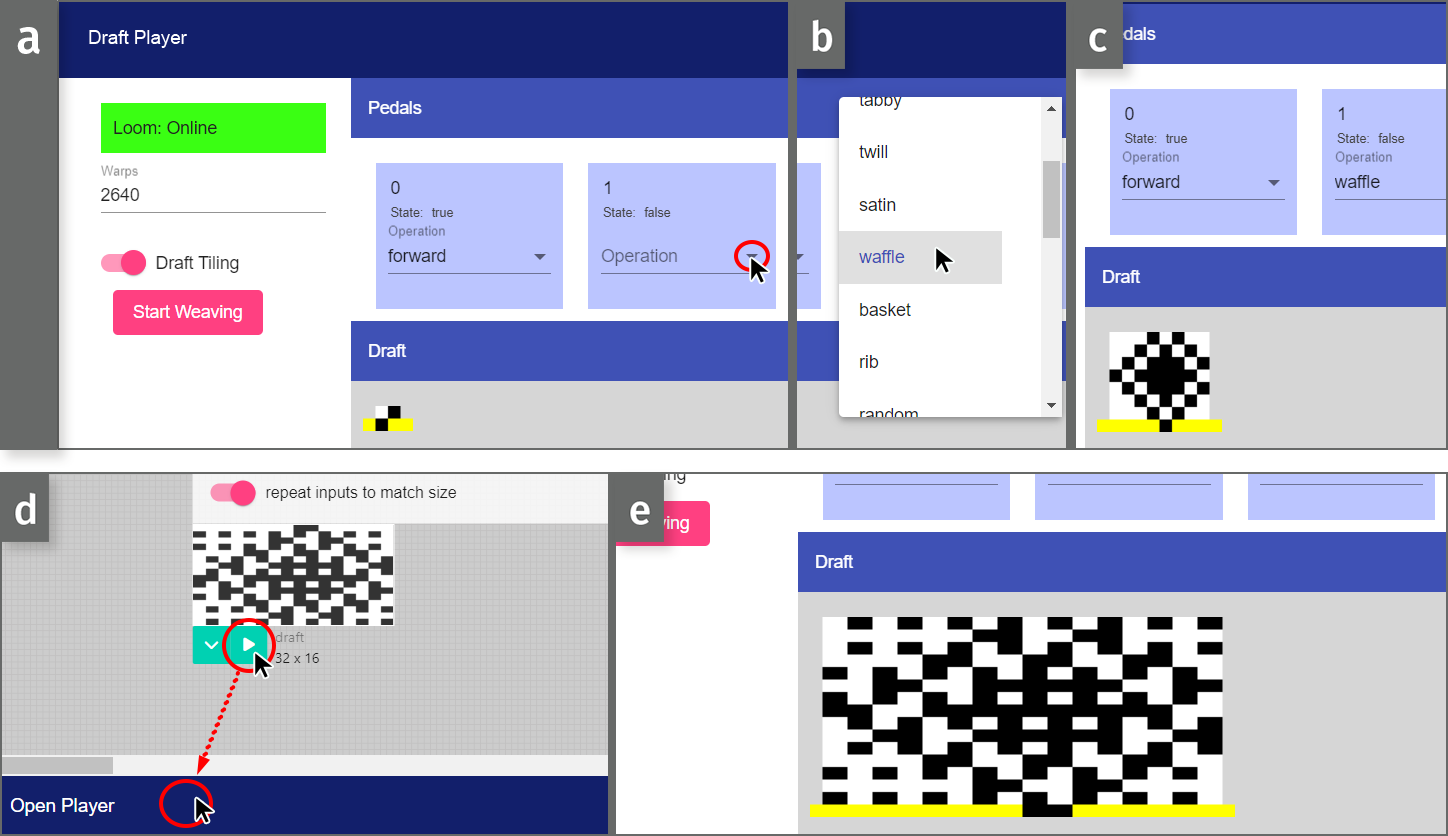
\includegraphics[width=0.9\linewidth]{figs/LP_gui_v2.png}
    \caption[Overview of the Draft Player, the Loom Pedals' interface in AdaCAD.]{Overview of the Draft Player, the Loom Pedals' interface in AdaCAD. a) The Player will start with a default tabby draft, and the first connected Pedal is automatically mapped to ``forward". b) Users can select an Operation to map to the Pedal. c) Any changes to the draft on the loom will be displayed, as well as the weaver's progress through the draft (yellow bar). d-e) Users can load a pre-made draft from the main AdaCaAD interface with a new ``Play" button.}
    \label{fig:draft-player-gui}
\end{figure}

Users can start directly in the Draft Player with one of the several basic building block drafts, as shown in Fig. \ref{fig:draft-player-gui}a--c. However, if they have prepared a draft in the Mixer, they can transition to the Player by clicking the Play button on a selected draft node (Fig. \ref{fig:draft-player-gui}d), which then loads the draft into the Player (Fig. \ref{fig:draft-player-gui}e). The Draft Player will display the number of Loom Pedals currently connected and some basic loom configurations, such as the number of warps on the loom. Each Pedal displayed has an associated menu of Operations the user can map to it. Most are ported over from AdaCAD’s existing Operations, with the exception of three Player-specific Operations which represent the user’s progress through the draft: forward, reverse, and refresh. The first two Operations are equivalent to basic functions in the TC2 software that let a user progress forwards/backwards in a draft. Meanwhile, the refresh Operation lets a user repeat the current row of the draft without progressing.

\section{Evaluation}

Our prototype represents a flexible constellation of hardware and software components in conversation with each other, with myself acting as the facilitator during initial implementation. Fittingly, our subsequent testing would also consist of conversations, now between people, about the affordances of the design. To evaluate the prototype, we considered its application in actual weaving practices and collaboratively reflected upon our experiences using the Loom Pedals, providing insights about further developments, and in a broader sense, weaving improvisationally.

\subsection{Recruiting Collaborators}

Following the initial Loom Pedals prototype, collaborators were recruited to gain insight into how the Pedals might provoke new ideas and what additional features our prototype needed to accommodate other weavers’ practices. We recruited weavers who also had some knowledge of physical computing, coding, or digital fabrication, to minimize the amount of onboarding necessary for understanding the Loom Pedals and modifying the prototype. Consequently, we agreed the weavers would be recognized as co-authors, to include them as active voices in shaping the design, questioning conventional divisions between researchers and participants, or developers and users.

\begin{table}
 \caption{Comparison of the Loom Pedals authors' weaving experiences and disciplinary backgrounds.}
 \label{table-authors}
 \begin{tabular}{r|c|c|c|c|c|c}
 \toprule
   Author & S (me) & Tom & Fram & Wren & Cece & Olive \\ \midrule
   {TC2 experience?} & $\checkmark$ & $\times$ & $\checkmark$ & $\times$ & $\times$ & $\checkmark$ \\
   {Background} & engineering & design & textiles & CS & engineering & CS \\
   {Years weaving} & 5 & 0$^\ast$ & 10 & 15 & 0$^\ast$ & 5 \\
   \bottomrule
   \end{tabular} \\ \vspace{0.5em}
   
   \footnotesize{$^\ast$ Tom and Cece began learning to weave at the start of the collaboration.}
\end{table}

\subsection{Procedure}

Over the course of 4 months in 2022, I met with each collaborator, in at least one session that lasted between 2 and 3 hours. These meetings had three parts: 1) a semi-structured interview, 2) a guided tutorial of the Loom Pedals interface followed by open weaving time, and 3) an in-depth discussion of each other's weaving practices. These sessions were audio-recorded from beginning to end.

The interviews consisted of a short list of prepared questions targeting the author's use of weaving tools, their interest in the TC2/Loom Pedals, as well as the values embedded in their design processes. During the tutorial, I prompted the other author to preview several simple structures using different transformations, until they settled on a starting draft. With yarn in hand, we then began weaving, allowing the collaborator to iterate on the loom for as long as they wanted. Once they finished, I asked them to share feedback regarding how they might use the Loom Pedals and what features would be helpful in implementing those uses. 

Afterwards, I transcribed the sessions, identifying key traits within each participant, such as: their relationship with improvisation while weaving, their use of reference materials, and how they learned new techniques. The draft samples were also analyzed (Fig. \ref{fig:author-samples}, accounting for which Operations were most provocative and what physical actions each author took to produce the sample. 

In addition to these collaborative sessions, I also conducted an extended test of the Loom Pedals by using the prototype for a multi-day, large-scale weaving. Their design and weaving process were recorded in multiple ways: a timelapse video, a screen recording of the Draft Player while weaving, and real-time videos of key moments e.g. when a special technique was used. The fabric shown in Figs. \ref{fig:teaser} and \ref{fig:example-workflow} is the result of this test.

We acknowledge that this work's autobiographical approach comes with its own limitations, like generalizability, discussed by Desjardins \& Ball \cite{desjardins_revealing_2018}. These open questions present opportunities for further research with the Loom Pedals; while the prototype serves as the foundation for any probes we may deploy. In the near future, we plan to reach out to a broader community of weavers, first locally, then to other spaces working with TC2s.

\section{Findings: Improvisational Weaving with the Loom Pedals}

Through my first-person design and use of the Loom Pedals, as well as collaborative sessions between the authors, we came to better understand the design space of improvisational weaving, and how the Pedals participated within that design space. We organize this section by highlighting the key findings, with narratives supporting each.

\begin{figure}
    \centering
    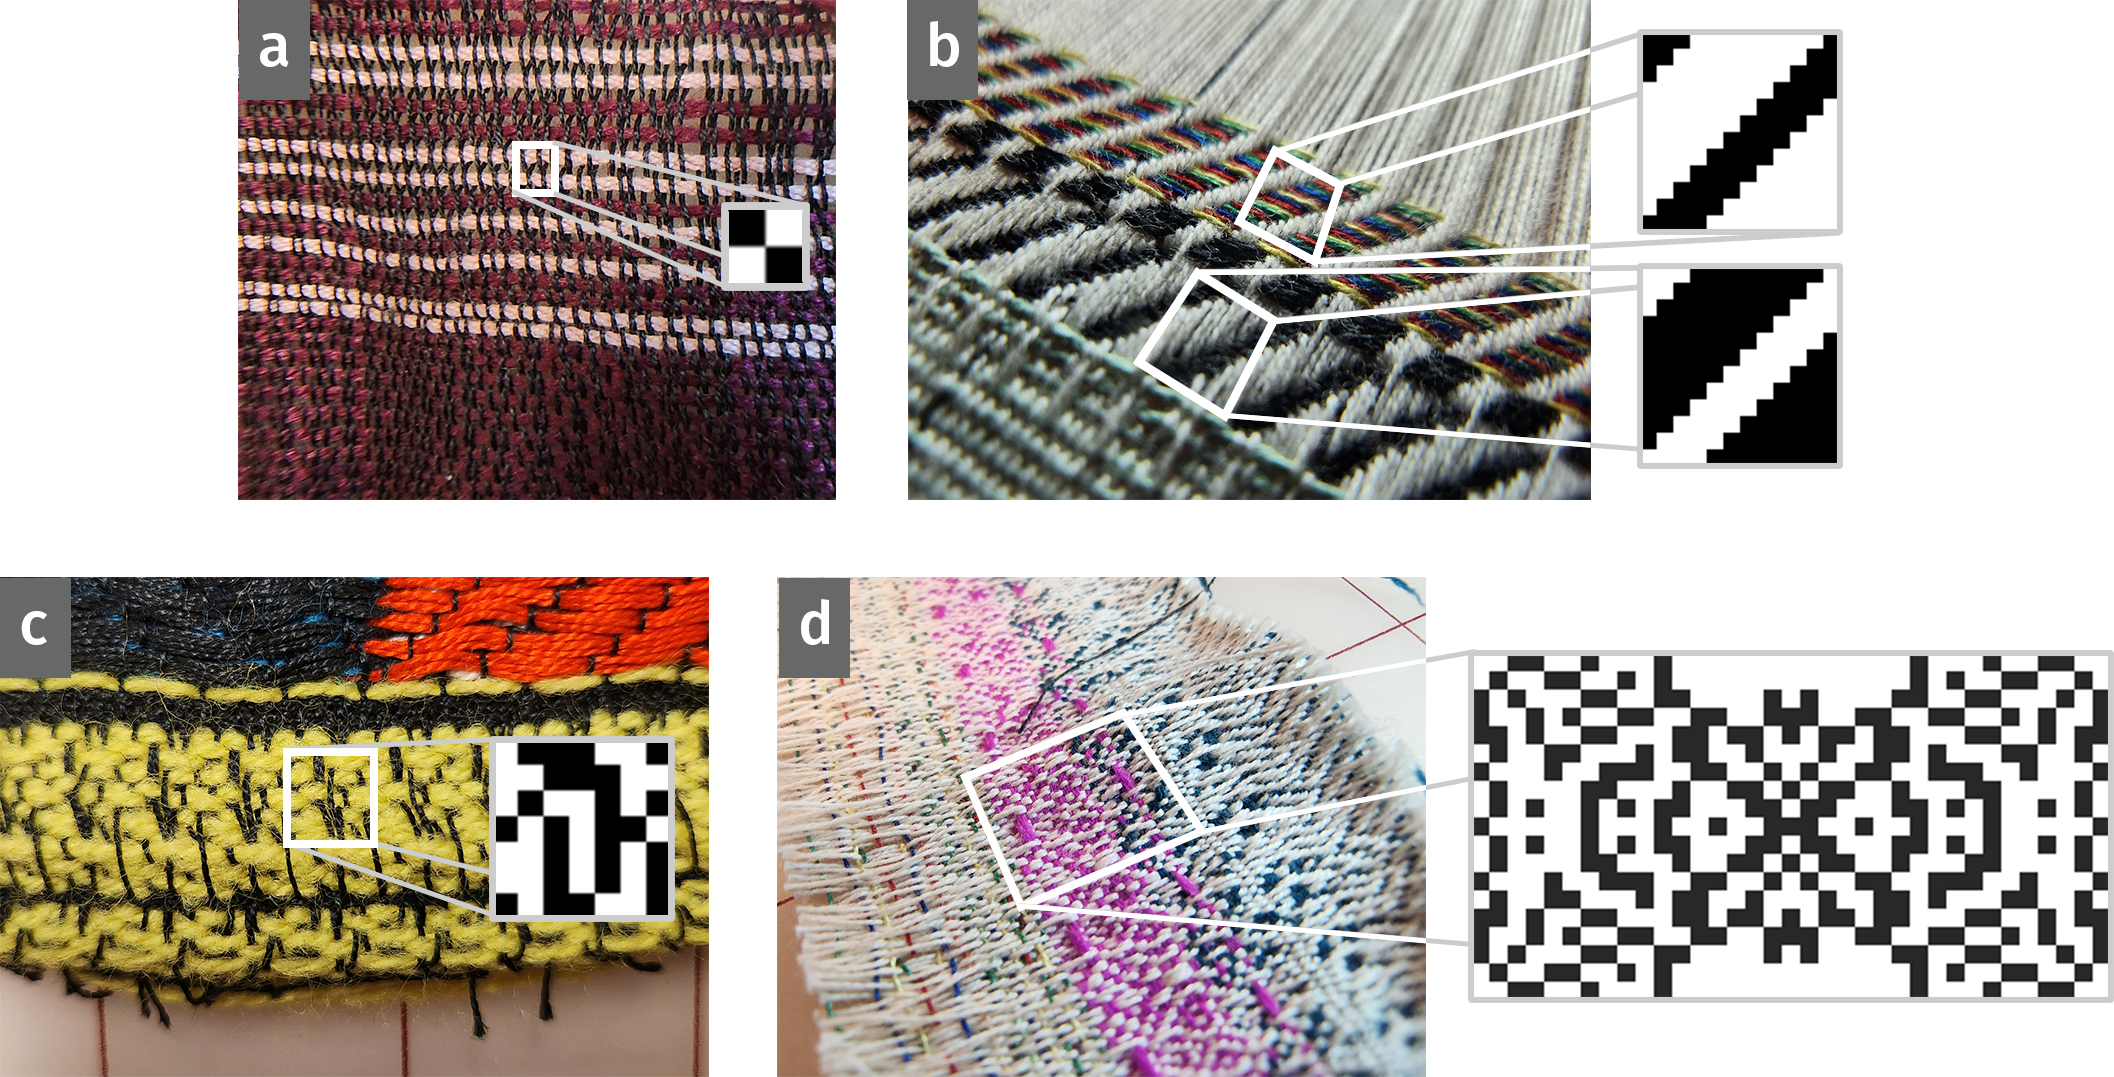
\includegraphics[width=\linewidth]{figs/LP_author-samples.png}
    \caption[Samples woven with the Loom Pedals and TC2.]{Samples woven with the Loom Pedals and TC2 by the authors, shown with the repeating draft of the woven structure. a) Cece's first try on the TC2, exploring tabby/plainweave and alternating colors. b) A large twill and its inverse woven by me. c) Wren's first try on the TC2, generating a small random draft. d) The results of Fram's experiments with a ``make symmetric" Operation to generate unique structures.}
    \label{fig:author-samples}
\end{figure}

\subsection{The Pedals Overcame Inertia and Provoked Happy Accidents}

I undertook the extended weaving test of the Loom Pedals as a personal challenge. In the past, they had abandoned similar TC2 projects because they did not have enough of an idea to fill the entire draft; they were stymied at the planning stages. With the Loom Pedals system at their disposal, they could finally gain some momentum. The draft began with a few basic weave structures before settling into a waffle weave
% \todo{(Fig. Xa draft view of basic waffle weave)}
, due to its contrast in texture and color. 

During the first few hours, I focused on trying different yarns with various waffle weave structures. One Pedal was set to waffle and three more to forward, refresh, and reverse, so the draft could be flexibly traversed. Two more Pedals were assigned stretch and invert operations to produce the variations
% \todo{(Fig. pedal configuration screenshot in figure)}
. At one point, I accidentally reassigned a Pedal to generate a random draft structure and altered the design drastically. I decided to embrace the mistake as a ``happy accident", and switched to a contrasting yarn to further highlight the change. 
% \todo{(Fig. Xb)}.

Eventually, one of the stretched waffle variants took hold as the main fabric structure. Afterwards, I stopped the loom to save this structure as the base draft, generated a few more variations in AdaCAD 
% \todo{(Fig screenshot of mixer palette)}
, and reconfigured the Pedals to load these new drafts before they resumed weaving. During my break, I realized that I could use waffle weave squares as "pixels" for a contrasting overlay 
% \todo{(Fig. Xc photo of squiggles)}
. I intertwined these pixels back and forth while weaving the base draft. A colleague would later see the squiggle effect and wondered if a twill structure could create a similar squiggle, informing another experiment later in the piece. 

\subsection{Interactions Felt Musical}

Across the collaborative sessions, all of the authors referenced musical practices at least once. While not all of the authors had experience playing an instrument, music was a part of all of our felt experiences and thus, made an easy reference point. When giving the tutorial, I found myself explaining the Loom Pedals by comparing the system to effects pedals, e.g. reverb. For Tom, their experience in audio software led to the Sequencer design in Section \ref{sect_poss-features}. Another conversational thread came from Wren, who was unfamiliar with improvisation in weaving, but drew analogies to performing improvisational music such as live jazz.

I had experience as an amateur musician, and also felt the musicality of the Loom Pedals during their extended test. Following the initial period of discovery previously described, I wove the rest of the piece in a cyclical process: starting with an idea, weaving different motifs based on that idea until one stood out, and repeating this new structure to complete the work. This workflow recalled my experiences jamming on a violin or playing the drums, beginning with a base beat or leitmotif and evolving from there. In the end, my improvisations with the Loom Pedals totaled 20 hours of weaving, over the course of 5 days. During the interim, my mind still mulled over the fabric's emergent design, like how music lingers in the ears after a long period of playing. I was brainstorming new possibilities and reflecting on the work I had already done: what could improve, what could change. 
% All told, they found the experience exhilarating, ripe with explorative potential. 

Working on the Loom Pedals design felt comparable to musicians wiring custom filters or building their own synths. Just like how weavers build looms from repurposed material or bolt attachments onto their loom frames, there was a kinship in this sort of hacking, as part of a larger culture of creative expression, improvisation, and reconfiguration \cite{facebookgroup_weaving_nodate, scoates_brian_2013}.

\subsection{Improvisation Required Learning and Unlearning}

Weaving is a repetitive activity, physically and cognitively. Much of a weaver’s learning process involves training their muscle memory and adjusting their workspace as needed. Once these actions become familiar gestures, the weaver enters a structured dance between themselves, the loom and the fabric. Consequently, those experienced with the TC2 develop strong personal preferences for how they arranged their tools, prepared materials, and moved around the loom. On positioning their foot pedal, Fram said that they ``preferred it to their right, near the [controller computer]" and would sometimes place a small dumbbell behind to prevent it from shifting. I differed, stating that they place the pedal ``in the center of the loom, so I can shift side to side while weaving and avoid locking my knees." 

Experience establishes these kinds of proclivities that aid in fluency; however, solidifying habits can also hinder play. To illustrate, Fram compared hand knitting with weaving at the TC2: “I find knitting to be really improvisational for me because I know much less about it." Accustomed to the standard TC2 drafting workflow, they unconsciously resist changing their design while making it. “It’s harder for me to get loose with [weaving] in the same way I do with knitting—add some stitches here, make this lumpy bit here." In contrast, as someone new to both knitting and weaving, Cece’s lack of experience allowed them to approach these crafts with a fearless curiosity. In that sense, disrupting one's workflow, like with the addition of the Loom Pedals, can help encourage play simply by virtue of their novelty.

\subsection{Weavers Needed to Trust the Machine}

The TC2 has undeniable agency when working with it. In the case of Wren and Cece, as new users, its sheer physicality and complexity made the TC2 an intimidating presence. When asked why, Cece replied, “because it is a machine...it is not my hands." For someone primarily experienced in hand tools, like sewing needles, using the TC2 meant surrendering a great deal of control on their part. On the other hand Wren had used shaft looms before and so they were comfortable entrusting the patterning and warp manipulation to the machine. They explained, “I just get [the loom] threaded, then play with the patterns…the threading steers you to a cluster of [possibilities]." We chose to describe this relationship between weaver and loom as trust, to reflect how the embodied process of handweaving builds familiarity and intimacy with one’s tools. 

\section{Mapping Possible Features}
\label{sect_poss-features}

Based on our collective testing, along with the insights from our interviews, we identified a number of possible features that could expand the expressive range of the Loom Pedals. We present these ideas in three broad categories, determined by how each feature increases possible inputs to the Pedals system. The categories are as follows: draft inputs, physical inputs, and time-dependent inputs. These classifications also define three axes of the Loom Pedals' design space for improvisational Jacquard weaving.

\subsection{Draft Inputs: Remixing and Emulating}

\begin{figure}
    \centering
    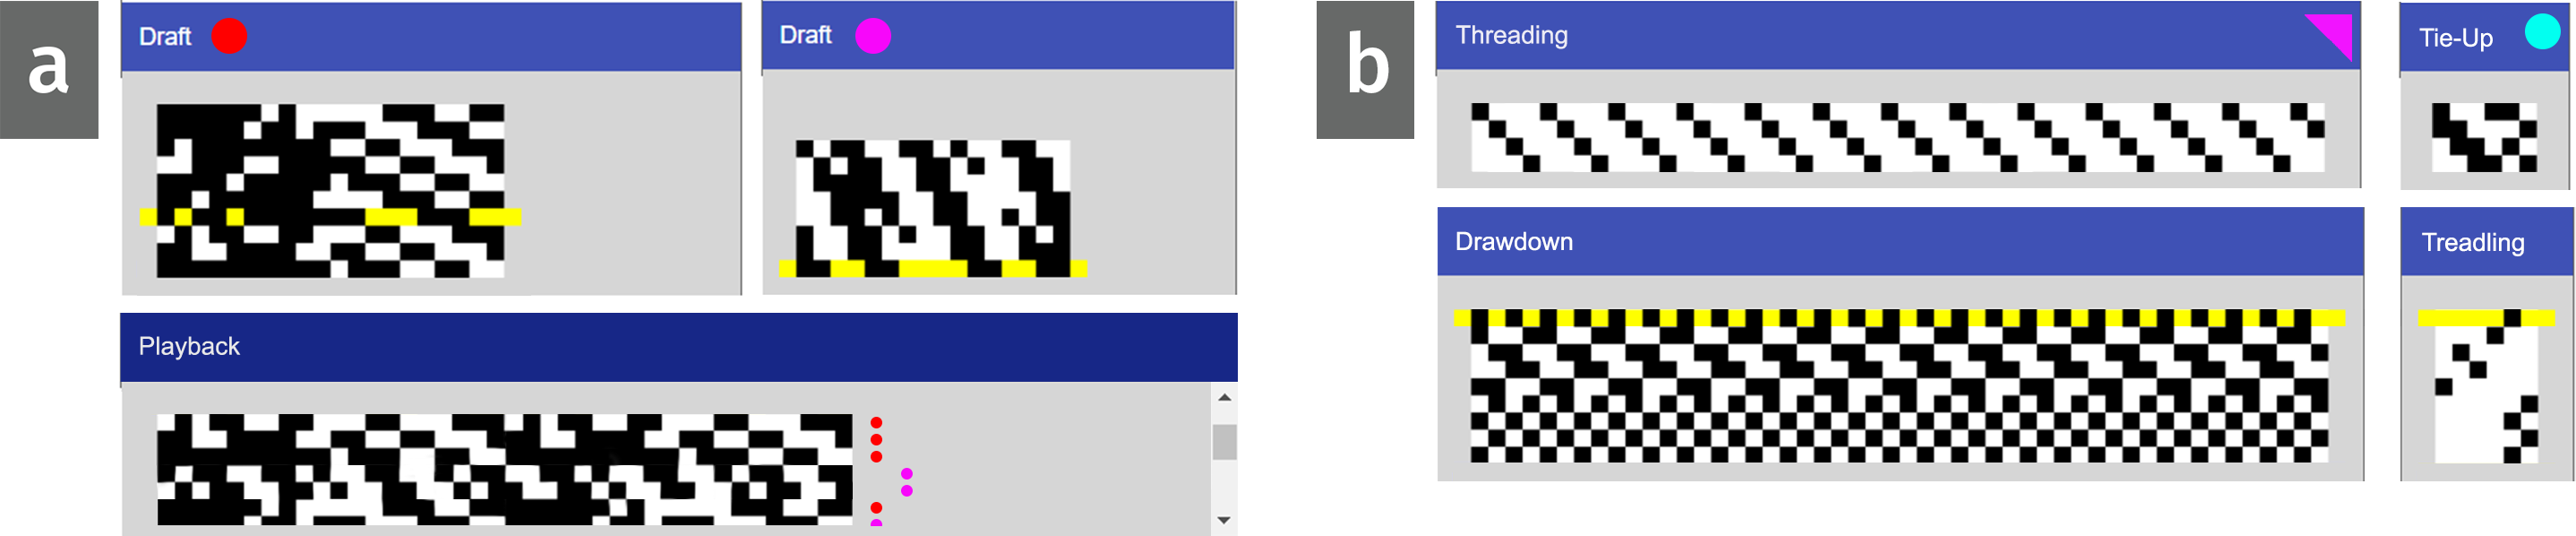
\includegraphics[width=\linewidth]{figs/LP_fig_draft-inputs.png}
    \caption[Key differences in AdaCAD with Remixing and Treadle features.]{Key differences in the software interface when using the Remixing and Treadle features. a) Remixing: Pedals are divided between the Drafts in the mix. The forward/reverse pedal for each Draft is highlighted in yellow. A ``Playback" component has been added underneath the Drafts, which also indicates which Draft each row was selected from. b) Treadles: Pedals that are configured as Treadles are grouped and condensed into a separate component from the Pedals that execute Operations.}
    \label{fig:remixing-emulating}
\end{figure}

Currently, the Loom Pedals prototype can handle one Jacquard draft at a time. However the system can be modified to handle multiple drafts, treating each as a separate track to remix while weaving (Fig. \ref{fig:remixing-emulating}a). The connected Pedals would be divided amongst the different drafts, each following a separate progression through set Operations. A new Playback component could record each row woven, highlighting when the weaver alternated between drafts. 

We can also consider how the Loom Pedals might handle non-Jacquard drafts, such as shaft loom drafts (see Fig. \ref{fig:drafts}). To use another technological analogy, we can turn the TC2 into a shaft loom emulator, as shown in (Fig. \ref{fig:remixing-emulating}b). The user would connect one Pedal per treadle. Additional Pedals could be connected to apply Operations during weaving. However, instead of applying the Operation to the drawdown, these Operations are applied to either the threading or tie-up, augmenting the flexibility of traditional shaft looms.

\begin{figure}[t]
    \centering
    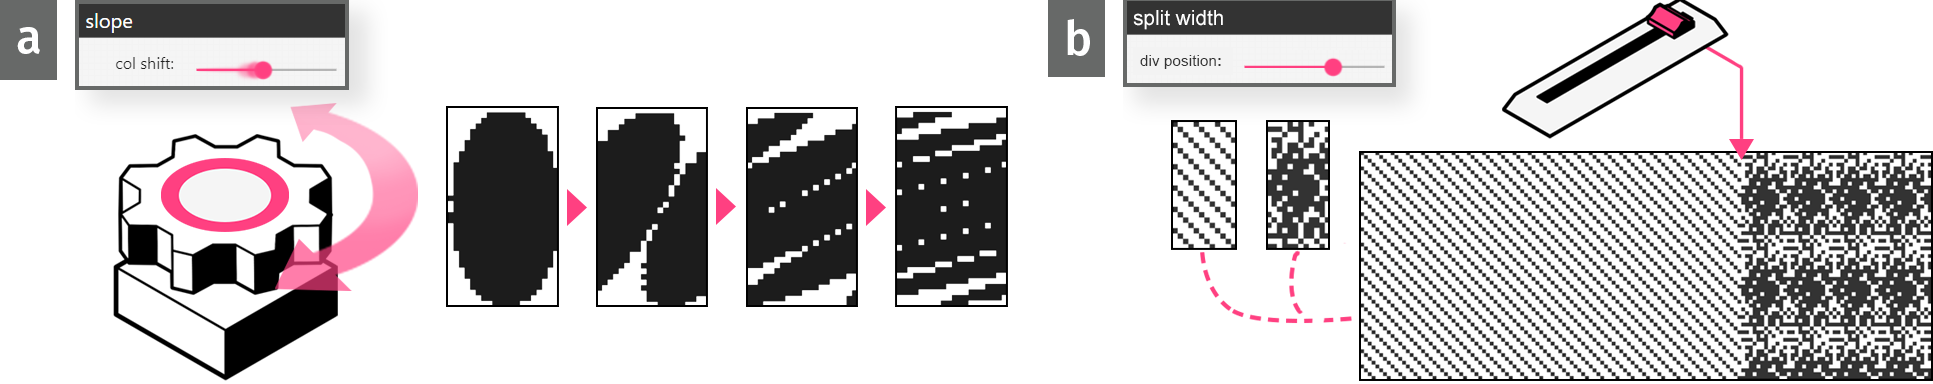
\includegraphics[width=\linewidth]{figs/LP_11_sliders.png}
    \caption[Two examples of how analog inputs might control weaving Operations.]{Two examples of how analog inputs might control weaving Operations. (a) A knob that the weaver turns to adjust the ``column shift" parameter of the Slope Operation. (b) A slider that allows two different drafts to be woven side-by-side, where the slider’s position corresponds to divisions in the weaving rows. Slider and gear icons by Lluisa Iborra from the Noun Project.}
    \label{fig:sliders-knobs}
\end{figure}

\subsection{Physical Inputs: Sliders and Knobs}

While our prototype only incorporates foot-controlled Pedals, we realized that hand-activated inputs would also fit into the rhythmic flow of weaving. For example, a user might prefer to press a button or keyboard to select an Operation. Beyond binary on/off inputs, we can also consider analog inputs like sliders and dials. In Fig. \ref{fig:sliders-knobs}, we present two examples of how analog inputs can be combined with parameterized Operations to enable even more responsive draft editing. This feature draws upon our experiences with hand tools like crochet hooks and manual weaving techniques, as we found ourselves wanting a direct connection with the materials. 


\subsection{Time Inputs: the Operation Sequencer}

\begin{figure}[h]
    \centering
    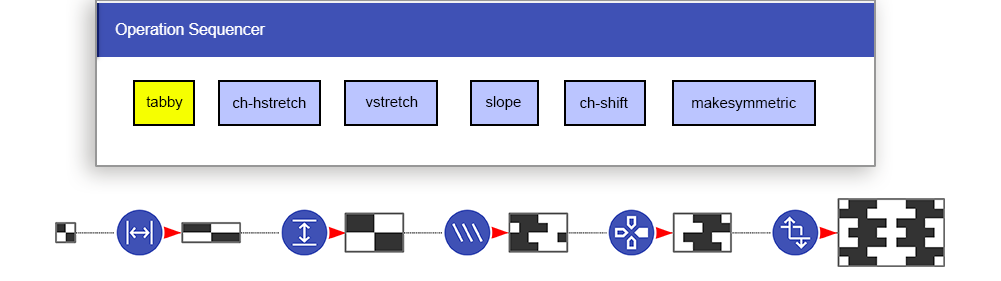
\includegraphics[width=\linewidth]{figs/LP_sequencer.png}
    \caption[The Operation Sequencer in the modified AdaCAD interface.]{An example configuration for the Operation Sequencer, a new section in the Draft Player. (top) The Sequencer has been loaded with the following Operations to execute from left to right: tabby structure, (chain) horizontal stretch, vertical stretch, slope, (chain) shift right, make symmetric. The ``hstretch" and ``shift" stages are chain Operations to perform a single transformation multiple times. (bottom) The Draft Player output as the Sequencer progresses.}
    \label{fig:sequencer}
\end{figure}


Lastly, we delved into how the Loom Pedals might evolve past base AdaCAD Operations. Generating a draft while weaving, instead of using CAD software before weaving, introduces a time component to Jacquard drafts. When no longer confined to a static image, a legacy of the punch-card, we can reimagine Jacquard drafts as a sequence of dynamic Operation inputs. In Fig. \ref{fig:sequencer}, we show the Operation Sequencer interface component, which we designed to enable more complex Operation mappings to the Loom Pedals. Not only can the user chain together Operations to act as a single transformation, they can also add Operations to the Sequencer, a queue of Operations, to apply at certain time intervals.

\section{Discussion}
\label{sect-discussion}

Looking back on our design and development process, we reflect on our original inquiry, the lessons learned, and how these insights will guide future development of the Loom Pedals. Primarily, we learned about the experience of improvising in the realm of textile craft, specifically weaving. Although, we focus our discussion on the unique facets of this project as they relate to broader discussions of improvisation and playful, creative interactions in the ubiquitous computing and HCI communities.

\subsection{Playful Peripherals for Digital Fabrication}

As discussed, one of our primary goals in designing the Loom Pedals was reimagining the TC2 workflow in ways that invited playful improvisation. Besides the insights we gained in the context of weaving, we found connections to other works investigating playful improvisation in the HCI community, particularly in digital fabrication. 

As technologies such as 3D printers and laser cutters become increasingly accessible to the general populace, these machines have also become sites for exploring interactions with fabrication, physical materials, and data. [general cite of interactive fab?] Research projects often build bespoke machines, such as a wall-sized vertical plotter \cite{cheng_duco_2021}, or augment existing systems with new sensors and input modalities to enable novel interactions [cite examples]. The Loom Pedals prototype does neither; it is a peripheral to an existing Jacquard Loom that expands one of the TC2's current input modalities. We highlight this fact to emphasize peripheral devices as an avenue for further design explorations in digital fabrication.

What would adding foot pedals to a 3D printer look like? What interactive mechanisms in printers might one draw out and exaggerate as a result? If foot-based interactions have distinct influences on the user's experience \cite{velloso_feet_2015}, how might playing with your feet, rather than twisting knobs or pushing buttons, free the hands for other forms of participation? How would this whole-body modality affect what users fabricate with the machine, whether for prototyping or creative expression? Without building a novel machine or introducing new sensors, bringing a sense of play to existing fabrication machines through peripheral devices, can unlock unique interactions and design opportunities.

\subsection{Generating Features Through Metaphor}

Next, we reflect on the two related metaphors which informed the design process: \textit{weaving as music} and \textit{weaving as conversation}. These metaphors not only helped clarify the design, by providing a foundation for the hardware and user interface, but also fostered ideas regarding future implementations, and deepened our understanding of weaving as a whole. 

My personal experience with musical instruments and DIY musical electronics inspired the underlying design of the Loom Pedals, assigning them transformative Operations in the same way a musical effects pedal would add reverb. Comparing weaving to music also shaped the Draft Player by noting how weaving a draft is like playing a track. In making these comparisons, we observe how weavers and musicians both hack their tools as part of their creative practices, suggesting a more profound connection between the crafts than the analogies we have stated. 

Meanwhile, framing weaving as conversation draws attention to the role of the loom in the weaving process. Again in terms of music, our reflections suggest that the loom is less like a musical instrument and more a partner in a duet. Jacquard looms were created to automate lifting warps in complex patterns, which would otherwise be performed manually, by the weaver or an assistant. Since the loom is standing in for a human agent, we feel it appropriate to treat the loom as such, recognizing the input it provides on designs that emerge from improvisational weaving. Thus, drafts are the common language between the loom and weaver, each row transmitting a unit of complete fabric, representing this dialogue. 

In mixing these metaphors, we drew inspiration from disparate technologies to inform our designs, entangling histories and embodied knowledge with practical needs and physical engagements.

\subsection{Learning from Historical Technologies}

% On a related note of adding new components into existing environments, 
To close, we consider how our design process was informed by older forms of weaving. The Loom Pedals' design was heavily influenced by the design of shaft looms, and to a lesser extent, tapestry looms. Unlike most ``dated" technologies, for example gramophones or cassette tapes, traditional looms are not considered obsolete to contemporary weavers and still see use alongside modern looms. Thus, we believe that the Loom Pedals presents a case study in how a fabrication system can use history to inform its design, a case in which the existing technologies have a unique relationship with history.

In HCI, an ongoing research agenda is augmenting existing objects and spaces to enable connected interactivity \cite{marques_pervasive_2019, zeagler_where_2017}, including intimate contexts such as showering at home \cite{kwon_connected_2018}. We note that nearly two decades ago, Wyche et al. called for researchers to sensitize themselves to past tools and cultural values in their design contexts, particularly when developing technologies for the home \cite{wyche_historical_2006}. Beyond the fact that textile crafts are often associated with home settings, designing for both of these domains can involve intimate, body-based interactions. Generally, researchers understand that users of these augmented objects will be carrying over habits and associations in the form of embodied knowledge and cognition \cite{lingel_poetics_2016}. Thus, designing technology to sense and respond to these kinds of intuitions, such as how to hold horsehair for embroidery \cite{flanagan_tracing_2019} or how weather can elicit sentimental responses \cite{brueckner_embodisuit_2018}, can enrich interactive systems for users. In that sense, embodied knowledge is a kind of history inscribed into our bodies and communities, where past interactions with technology inform future behaviors. As such, historical technologies within our domain provide a wealth of possibilities for exploring new designs, rooted in older interactions.

By unlearning terms like outdated, obsolete, and low tech, we can reexamine modern problems through the lens of past designs. Because a majority of shaft loom usage was pre-industrialization, their mechanics offered a unique take on improvisation, distinct from newer Jacquard looms. This distinction helped anchor our initial ideation for how to reimagine the TC2 workflow and it guided us throughout the design process, as a point of reference. 


\section{Crafting Future Tools with the Past}
\label{sect-conclusion}

In summary, we began this chapter by discussing the state of Jacquard weaving in textiles design and prototyping, and the limitations of the current workflow, as it relates to other types of weaving, particularly weaving on traditional shaft looms. We reviewed recent developments in HCI, where researchers have developed digital fabrication tools that make fabrication techniques and hardware more accessible, expressive, and collaborative. Given the related research in digital fabrication, we saw opportunities to design alternative hardware and software interfaces for Jacquard weaving that centered on playful improvisation, rather than meticulous planning. Our contribution consists of the documentation of our design and prototyping process, findings in the form of design lessons, and the resulting open-source interface to the TC2 digital Jacquard loom.

To review, the Loom Pedals are a hardware/software system of modular, interchangeable pedal inputs for the TC2, one of the few commercially-available models of Jacquard loom accessible to consumers. The customizable interface allows a weaver to place as many Pedals as desired, assign functions to them, which dynamically generate and transform drafts, then begin weaving an emergent design with little to no preparation. As a mixed group of experienced and novice Jacquard weavers, our own weaving practices informed this prototype. 

First, we implemented the core functionality, then collaborated amongst ourselves to design additional features for the Loom Pedals, to accommodate our varied weaving experiences. Reflecting on the process of designing and using the Loom Pedals, we found common themes that influenced improvisation and play in our weaving practices. We present the collaboratively generated features as expansions to the Loom Pedals along three distinct axes of system inputs: draft inputs, physical inputs, and time-based inputs. Finally, we conclude with discussion points that relate to broader themes in the HCI research community. 

Ultimately, I see the Loom Pedals as a system which brings the machine, design data, and human weaver into a direct dialogue with one another---a dynamic echoed in a world which increasingly links virtual and physical agents, as well as humans and the more-than-human. I built the Loom Pedals in the later half of my PhD studies, after I had more fully developed an awareness of coproduction as an active influence in my craft. And at this point, I worked with our lab's specific TC2 for several years---wove with it, warped it with my labmates, climbed inside it to install new parts---and come to care for it as a research sibling. In addition to this machine relationship, this project also integrated relationships with other humans in developing and testing the Loom Pedals. After spending much of my PhD program in the midst of the COVID-19 pandemic, I had become extremely isolated in my crafting practice. Reconnecting with the human dimension of design gave me a hard reminder to maintain connections with \textit{all} beings in my ecosystem.

